%%%%%%%%%%%%%%%%%%%%%%%%%%%%%%%%%%%%%%%%%%%%%%%%%%%%%%%%%%%%%%%%%%%%%
%%%                       ANALYSIS OVERVIEW                       %%%
%%%%%%%%%%%%%%%%%%%%%%%%%%%%%%%%%%%%%%%%%%%%%%%%%%%%%%%%%%%%%%%%%%%%%
\section{Analysis overview}
In this analysis we are searching for a signal of possible neutrino magnetic moment events in the NOvA Near Detector. This signal would manifest as an excess of neutrino-on-electron elastic scattering ($\nu$-on-e) events at low electron recoil energies on top of the Standard Model background, as described in Sec. \ref{sec:MeasuringNuMM}. In case we would not observe any excess (null hypothesis), we would provide an upper limit on the effective muon neutrino magnetic moment.

The $\nu$-on-e interactions are also used in the Near Detector (ND) group's analysis to constraint the neutrino beam prediction \cite{NOVA-doc-56383}, which relies on the precise theoretical knowledge of the $\nu$-on-e interaction cross section. They compare the total number of recorded $\nu$-on-e interactions, with background subtracted based on a data/MC comparison in a sideband region, to the prediction. Since the number of $\nu$-on-e events should only depend on the normalization of the neutrino beam, this analysis should give us a precise validation, or correction, of the neutrino flux normalization. There has been a large amount of work going into this analysis, including making special samples, weights, event classifiers, developing a dedicated event selection, or developing a background subtraction method, among others. To save time and analysis effort, we have taken most of these work at face value and applied it to the neutrino magnetic moment analysis. This will help us get the first good estimate of NOvA's capabilities to constraint (or measure) the neutrino magnetic moment.

The same detector signature of a single forward going electron shower, as present in the $\nu$-on-e events, is also present in the Light Dark Matter (LDM) analysis \cite{NOVA-doc-59439}. This analysis is using a similar event selection to select the LDM events as the ND group, only without the final $E\theta^2$ cut (see Sec.\ref{sec:EventSelection}). However, instead of simply comparing the total event counts, the LDM analysis is using a CAFAna-based fitting framework to fit for the possible LDM signal in a distribution of electron recoil energy multiplied by electron recoil angle squared.

%What are we trying to achieve? We are trying to see the low energy excess of very forward neutrino-on-electron ($\nu$-on-e) events. We can either do this via a counting experiment (possibly with various control samples/regions to control backgrounds and systematics), or with a fit to the energy spectrum of well-selected $\nu$-on-electron events.

Our analysis strategy is to compare the recorded number of neutrino events in data with a predicted number of signal events, which depends on the neutrino magnetic moment value, on top of a Standard Model background. We use the ND group's sideband region to constraint the non-$\nu$-on-e background with data. It is also possible to use a second sideband sample, based on the electron recoil energy, to provide an additional constraint on the $\nu$-on-e background, but this idea has not been visited yet.

In the future, this analysis can be improved for example by improving the event selection, creating additional background samples, by including antineutrino events, or by using using a fit to the energy distribution, similarly to the LDM analysis.

This section describes the simulation samples used to predict the number of signal and background events (Sec.\ref{sec:datasets}), the weights used to correct for known limitations of the simulation (Sec. \ref{sec:anaWeights}), the event selection used to constraint the background (Sec. \ref{sec:EventSelection}), and the resolution of the electron recoil energy and angle (Sec. \ref{sec:resolution}).

% Not sure if this should be here or in the datasets subsection... Here on forward I'm going to describe the differences between these (definitions, weights, signal def, systematics. What is the same: event selection and binning. They're joint together in the fitting framework, where the $\nu_e$CC MEC and the other backgrounds are simply summed together and scaled together. The $\nu$-on-e background (also called the irreducible background by the LDM analysis) is treated/scaled separately.

\subsection{Datasets and Event Reconstruction details}\label{sec:datasets}
For this analysis we are using near detector CAF samples with the standard Production 5.1 reconstruction.

The SAMWEB definition for the data sample is:
\begin{center}
\texttt{prod\_caf\_R20-11-25-prod5.1reco.l\_nd\_numi\_fhc\_full\_v1\_goodruns}.
\end{center}
We are following the standard data blinding procedure and have not looked at any data events until the analysis passes the full collaboration review. The Near Detector group has validated \todo{Figure out where did Yiwen and Wenjie actually look at the data} using this data sample.

The exposure of the data sample is approximately $1.3848600\times 10^{21}\ \unit{POT}$. This is the exposure we use for all the following studies shown in this technical note.
The Prod5.1 ND data sample contains data from run 10391 in epoch1a (2014-08-22 21:08:40) until run 14010 in epoch 11a (2021-02-03 15:48:21) (from the period and epoch naming wiki page https://cdcvs.fnal.gov/redmine/projects/novaart/wiki/Period\_and\_Epoch\_Naming)

\todo{Briefly describe the MC details. Versions of the individual simulation software}
To tackle the low number of $\nu$-on-e and $\nu_e$CC MEC events in the nominal simulation sample we are using a suit of nominal and enhanced simulation samples for four different signal and background components. Each one contains its nominal sample and special systematically shifted samples for the detector systematics. The use of the samples is summarised in table \ref{tab:SignalDefinitions} and described in detail below.

The \textsf{GENIE} tune is \texttt{GENIE N1810j 02 11a} (from the Prod5.Frankenstein docdb: 53360).
The Genie release used for this production is R20-08-06-prod5.1genie.h, which has GENIE version V3.0.6 \cite{GENIE}

Also prod5.1 uses Geant4 v4.10.4.p02 \cite{Geant4}

We use the standard NOvA simulation (reference NOvA 3fl paper DOI: 10.1103/PhysRevD.106.032004)

Describe how did we deal with the GENIE skew fix. It was the GSF weights that forces "us" to treat the nueCC MEC background differently than the other background. As I understand it, the GSF is applied simply as the new weight. No change to the systematics is required.

Reference: A. Mislivic, “Genie skew reweight validation.” NOvA Internal Document, DocDB: 553811
[from antinueCC IncXSec docdb:53691]
"Final state kinematics were predicted by the N1810j 00 000 tune, but total cross section were generated with the intended N1810j 0211a179 tune, which differed in RES and DIS rates tuned to external data. Properly correcting the skew180 would require all simulation to be regenerated, so a temporary solution developed by the NOvA181 Cross-section Tuning Group involves reweighing production 5.1 events to the default N1810j 00 000.182 An additional modification to the GENIE MEC contribution are applied to better agree with NOvA183 ND data.

MC includes simulation in the rock surrounding the ND

\todo{Describe here that we're using the nominal ND MC sample for signal utilizing the simple relationship between the Standard Model cross section and the neutrino magnetic moment cross section (ref. theory)}

The signal of the neutrino magnetic moment analysis is just a re-weighted signal of the $\nu$-on-e analysis from the near detector group. We are using the same event selection as the near detector group.

\todo{Say already here that the POT inside the enhanced MC samples are not properly accounted for in CAFAna (Loader issue) and so the event counts need to be adjusted post-hoc}

\begin{table}[!ht]
\centering
\caption{Overview of the simulation samples corresponding to different signal and background components.}
\def\arraystretch{1.4}
\begin{tabular}{l@{\hskip 1in}l}
Signal                   & Enhanced $\nu$-on-e sample\\
$\nu$-on-e background    & Enhanced $\nu$-on-e sample\\
$\nu_e$CC MEC background & Enhanced $\nu_e$CC MEC sample\\
Other background         & Nominal ND CAF sample
\end{tabular}
\label{tab:DefinitionsOverview}
\end{table}

\subsubsection*{Enhanced $\nu$-on-e sample}
\todo{Describe the nuone sample}
Created by Wenjie Wu (was it just him or also Yiwen?) to do ... and fully described in the technote \cite{NOVA-doc-56383}. Using the overlayed and filematched samples for consistency.

Incorrect POT is 3.6995434e+20, Correct POT is 1.7209423e+24 (this should be filematched)

\todo{Find a reference and reasoning for why Wenjie hasn't created the other systematics samples}
We only have the selected few systematics definitions because ... 

\todo{Describe the differences}
\begin{itemize}
\item Missing cross section parameters - unable to use cross section weights or so
\item Special mode for nu-on-e elastic scattering 10005
\end{itemize}

The list of the nu-on-e sample definitions is in table \ref{tab:NuoneDefinitions}.

\begin{table}[!ht]
\centering
\caption{SAMWEB definitions for the enhanced $\nu$-on-e samples.}
\begin{tabular}{p{\textwidth}}
\hline\hline\\[-2mm]
\textbf{Nominal:}\\
\texttt{prod\_caf\_R20-11-25-prod5.1reco.g\_nd\_genie\_N1810j0211a\_nonswap\_fhc\_nova\_v08} \texttt{\_full\_v1\_nuone\_overlay}\\[7mm]
\textbf{Systematically shifted samples:}\\
\texttt{prod\_caf\_R20-11-25-prod5.1reco.g\_nd\_genie\_N1810j0211a\_nonswap\_fhc\_nova\_v08} \texttt{\_full\_calibup\_v1\_nuone\_overlay}\\[7mm]
\texttt{prod\_caf\_R20-11-25-prod5.1reco.g\_nd\_genie\_N1810j0211a\_nonswap\_fhc\_nova\_v08} \texttt{\_full\_calibdown\_v1\_nuone\_overlay}\\[7mm]
\texttt{prod\_caf\_R20-11-25-prod5.1reco.g\_nd\_genie\_N1810j0211a\_nonswap\_fhc\_nova\_v08} \texttt{\_full\_ckvup\_v1\_nuone\_overlay}\\[7mm]
\texttt{prod\_caf\_R20-11-25-prod5.1reco.g\_nd\_genie\_N1810j0211a\_nonswap\_fhc\_nova\_v08} \texttt{\_full\_ckvdown\_v1\_nuone\_overlay}\\[7mm]
\texttt{prod\_caf\_R20-11-25-prod5.1reco.g\_nd\_genie\_N1810j0211a\_nonswap\_fhc\_nova\_v08} \texttt{\_full\_lightlevelup\_v1\_nuone\_overlay}\\[7mm]
\texttt{prod\_caf\_R20-11-25-prod5.1reco.g\_nd\_genie\_N1810j0211a\_nonswap\_fhc\_nova\_v08} \texttt{\_full\_lightleveldown\_v1\_nuone\_overlay}\\[7mm]
\hline\hline
\end{tabular}
\label{tab:NuoneDefinitions}
\end{table}

\subsubsection*{Enhanced $\nu_e$CC MEC sample}
Created by Yiwen Xiao \cite{NOVA-doc-56383} to tackle the low statistics of the $\nu_e$CC MEC background events and subsequently large and unphysical cross section weights.

Incorrect POT is 4.7334120e+23 and correct POT is 1.9880340e+24. This is filematched

\todo{List the limitations of the sample in the q3-q0 parameter space}

\begin{table}[!ht]
\centering
\caption{SAMWEB definitions of the $\nu_e$CC MEC background sample.}
\begin{tabular}{p{\textwidth}}
\hline\hline\\[-2mm]
\textbf{Nominal:}\\
\texttt{YiwenXiao\_NueCCMEC\_Single\_NJobs7500\_CAF\_NonSwap\_filematch}\\[2mm]
\textbf{Systematically shifted samples:}\\
\texttt{YiwenXiao\_NueCCMEC\_Single\_NJobs7500\_CAF\_NonSwap\_CalibUp\_Combined\_240124\_filematch}\\[2mm]
\texttt{YiwenXiao\_NueCCMEC\_Single\_NJobs7500\_CAF\_NonSwap\_CalibDown\_Combined\_240124\_filematch}\\[2mm]
\texttt{YiwenXiao\_NueCCMEC\_Single\_NJobs7500\_CAF\_NonSwap\_CkvUp\_Combined\_240124\_filematch}\\[2mm]
\texttt{YiwenXiao\_NueCCMEC\_Single\_NJobs7500\_CAF\_NonSwap\_CkvDown\_Combined\_240124\_filematch}\\[2mm]
\texttt{YiwenXiao\_NueCCMEC\_Single\_NJobs7500\_CAF\_NonSwap\_LLUp\_Combined\_240124\_filematch}\\[2mm]
\texttt{YiwenXiao\_NueCCMEC\_Single\_NJobs7500\_CAF\_NonSwap\_LLDown\_Combined\_240124\_filematch}\\[2mm]
\texttt{YiwenXiao\_NueCCMEC\_Single\_NJobs7500\_CAF\_NonSwap\_Aging\_Combined\_240124\_filematch}\\[2mm]
\texttt{YiwenXiao\_NueCCMEC\_Single\_NJobs7500\_CAF\_NonSwap\_CalibShape\_Combined\_240124\_filematch}\\[2mm]
\texttt{YiwenXiao\_NueCCMEC\_Single\_NJobs7500\_CAF\_NonSwap\_MCNP\_Combined\_240124\_filematch}\\[2mm]
\hline\hline
\end{tabular}
\label{tab:NueCCMECDefinitions}
\end{table}

\subsubsection*{Near Detector filematched CAF sample}
\todo{describe all the ND nominal CAF samples}
\todo{Also mention the decaf sample and discuss if we could use them or not}

The nominal ND MC includes 4x data POT. The systematics are file-matched to remove any statistical bias

Total POT is 5.54497e+21
But for the filematched samples (batch 2) there's only 1.93109e+21

\begin{table}[!ht]
\centering
\caption{SAMWEB definitions of the other background samples.}
\begin{tabular}{p{\textwidth}}
\hline\hline\\[-2mm]
\textbf{Nominal:}\\
\texttt{prod\_caf\_R20-11-25-prod5.1reco.a\_nd\_genie\_N1810j0211a\_nonswap\_fhc\_nova\_v08} \texttt{\_full\_v1}\\[7mm]
\textbf{Systematically shifted samples:}\\
\texttt{prod\_caf\_R20-11-25-prod5.1reco.e\_nd\_genie\_N1810j0211a\_nonswap\_fhc\_nova\_v08} \texttt{\_full\_calibup\_v1\_batch2}\\[7mm]
\texttt{prod\_caf\_R20-11-25-prod5.1reco.e\_nd\_genie\_N1810j0211a\_nonswap\_fhc\_nova\_v08} \texttt{\_full\_calibdown\_v1\_batch2}\\[7mm]
\texttt{prod\_caf\_R20-11-25-prod5.1reco.f\_nd\_genie\_N1810j0211a\_nonswap\_fhc\_nova\_v08} \texttt{\_full\_ckvup\_v1\_batch2}\\[7mm]
\texttt{prod\_caf\_R20-11-25-prod5.1reco.f\_nd\_genie\_N1810j0211a\_nonswap\_fhc\_nova\_v08} \texttt{\_full\_ckvdown\_v1\_batch2}\\[7mm]
\texttt{prod\_caf\_R20-11-25-prod5.1reco.g\_nd\_genie\_N1810j0211a\_nonswap\_fhc\_nova\_v08} \texttt{\_full\_lightlevelup\_v1\_batch2}\\[7mm]
\texttt{prod\_caf\_R20-11-25-prod5.1reco.g\_nd\_genie\_N1810j0211a\_nonswap\_fhc\_nova\_v08} \texttt{\_full\_lightlevelup\_v1\_batch2}\\[7mm]
\texttt{prod\_caf\_R20-11-25-prod5.1reco.f\_nd\_genie\_N1810j0211a\_nonswap\_fhc\_nova\_v08} \texttt{\_full\_detectorageing\_v1\_batch2}\\[7mm]
\texttt{prod\_caf\_R20-11-25-prod5.1reco.f\_nd\_genie\_N1810j0211a\_nonswap\_fhc\_nova\_v08} \texttt{\_full\_calibshape\_v1\_batch2}\\[7mm]
\texttt{prod\_caf\_R20-11-25-prod5.1reco.g\_nd\_genie\_N1810j0211a\_nonswap\_fhc\_nova\_v08} \texttt{\_full\_mcnp\_v1\_batch2}\\[7mm]
\hline\hline
\end{tabular}
\label{tab:CAFDefinitions}
\end{table}

\iffalse
\subsubsection*{Near detector flat summed decaf sample}
What are the cuts used for the DeCAF sample? Why was it created? What is the effect of these cuts?

There's also 3 flavour concats - what are those? there are both numu and nue and they're for the ND... What are the cuts used to create these?

Should I include here also why did I choose to use the decafs instead of cafs? Maybe just point to my talks where I show the plot how much faster it is and that it doesn't matter much for the result. Maybe discuss how different the result would be if I used cafs instead of decafs...
\fi

\subsection{Analysis weights}\label{sec:anaWeights}
\todo{Describe why do we use weights}
What are the weights we are using and why?

To correct for known deficiencies in simulation of neutrino flux or cross sections we apply weights calculated for each event.

Table \ref{tab:WeightsOverview} shows what CAFAna weights are used to simulate what signal/background sample.

\begin{table}[!ht]
\centering
\caption{Overview of CAFAna weights applied to each analysis sample.}
\def\arraystretch{1.4}
\begin{tabular}{l@{\hskip 1in}l}
Signal                   & Flux and neutrino magnetic moment weights\\
$\nu$-on-e background    & Flux and radiative correction weights\\
$\nu_e$CC MEC background & Flux and cross section weights\\
Other background         & Flux and cross section weights
\end{tabular}
\label{tab:WeightsOverview}
\end{table}

\subsubsection*{PPFX weight}
\texttt{ana::kPPFXFluxCVWgt} \cite{NOVA-doc-23441}
\todo{What does this do (one sentence ish).}
Maybe cite Leo's thesis? Or paper?
L. Aliaga, “Neutrino Flux Prediction for the NuMI Beamline.” PhD Thesis, FERMILAB-1081
THESIS-2016-03


\subsubsection*{Prod5.1 GSF XSec weight}
\texttt{ana::kXSecCVWgt2020GSFProd51}
\todo{Find the reference: possibly Maria's docdb:53336 together with the official 2020 XSec tuning technote docdb:43962.}

NOvAReweight reference: J. Wolcott, “NOvARwgt software.” https://github.com/novaexperiment/NOvARwgt-public.

\todo{Briefly describe what does this do. Also mention Yiwen's talk/technote about the large XSec weights that made her create an enhanced nueCC MEC sample.}

We are only using the for the background since we assume that the cross section for the signal is perfect. Also there are not weights for this kind of interaction.

\subsubsection*{Radiative correction weight}
\todo{Why are we doing this? (reference Yiwen's talk/technote).}

Mention here where did I get the original GENIE cross section from (reference Yiwen's talk or technote, plus the original paper that was used). nu-on-e technote\cite{NOVA-doc-56383}

\todo{Write out the actual version of the weight. Including the original and the corrected XSec constants}

MINERvA paper:
https://journals.aps.org/prd/pdf/10.1103/PhysRevD.100.092001

Say that we are not using the third part of the correction because it is tiny and it makes no difference. (tried and tested)

\todo{correct the equation}
Calculated as 
\begin{equation}
weight_{\text{Radiative Corr.}} = \left.\frac{d\sigma_{\nu-on-e}}{dy}\right|_{\text{Radiative Corr.}} / \left.\frac{\textsf{d}\sigma_{\nu-on-e}}{\textsf{d}y}\right|_{\text{GENIE 3}};\,y=\frac{E_e-m_e}{E_\nu}
\end{equation}

\subsubsection*{Neutrino magnetic moment signal as a weight}
\todo{What does this do and why does it work? Reference the theory part as to why is the magnetic moment signal simply a rescaling of the GENIE cross section.}

Using the same tree-level cross section from GENIE as in the rad. corr. weight.

\todo{Write the name of the weight in CAFAna/nuone namespace and where it is located}

\todo{correct the equation}
Calculated as 
\begin{equation}
weight_{\nu\text{ Mag. Moment}} = \left.\frac{d\sigma_{\nu-on-e}}{dy}\right|_{\nu\text{ Mag. Moment}} / \left.\frac{\textsf{d}\sigma_{\nu-on-e}}{\textsf{d}y}\right|_{\text{GENIE 3}};\,y=\frac{E_e-m_e}{E_\nu}
\end{equation}

\subsection{Event selection}\label{sec:EventSelection}

We are trying to select low energy neutrino-on-electron events, which are characterised by a single very forward going electron shower. Since these are the same events as are used in the Near Detector group's analysis to constraint the neutrino beam prediction with a neutrino-on-electron events \cite{NOVA-doc-56383}, we have taken taken their event selection without changes. This is to save time and analysis efforts, but also to get a first good estimation of NOvA's capabilities to constraint (or measure) neutrino magnetic moment. Almost the same selection is also used in the Light Dark Matter analysis \cite{NOVA-doc-59439}, only without the final $E\theta^2$ cut.

We explain the motivation behind each cut of the event selection and discuss their effect on the neutrino magnetic moment events below. We also consider possible improvements to the event selection for a future (re-)analysis.

The code to make plots and analyse the event selection is located in the \path{NuMagMomentAna/NuMMAnalysis/EventSelection} directory. The signal definition is in \path{NuoneCuts.h} and the cut values in the \path{EventCVNCuts.h/cxx} scripts from the \path{NuMagMomentAna/Cuts} directory.

\subsubsection*{Signal definition}
To define the signal and background samples we use the true information listed in table \ref{tab:SignalDefinitions}. The neutrino magnetic moment signal definition is the same as the neutrino-on-electron background with the neutrino magnetic moment weight applied, as explained in sec.\ref{sec:anaWeights}. 

The signal definitions use the $kMode$ variable instead of the $kIntType$, which is now deprecated (ref.: various Slack conversations). Mode 10005 denotes only the $\nu$-on-e events and is only available for the enhanced $\nu$-on-e samples, while mode 5 denotes all electron scattering events, including inverse muon decay interactions. That is why we had to add a requirement of an electron in the final state. Mode 10 denotes all Meson Exchange Current (MEC) events.

We are using the ND group's \cite{NOVA-doc-56383} signal definition including a requirement for the true vertex to lie within their fiducial volume (defined below). This is the cut name \texttt{NDNuoneFiducial}. This is in contrast with the LDM analysis \cite{NOVA-doc-59439}, which uses the \texttt{ana::kVtxIsContained} cut instead, which has a looser boundary. This choice has only a negligible effect on the final number of selected events and only affects the selection efficiency.

\begin{table}[!ht]
\centering
\caption{Overview of signal and background definitions.}
\def\arraystretch{1.4}
\begin{tabular}{p{.25\textwidth}p{.7\textwidth}}
Signal                   & \texttt{kMode}== 10005 \&\& \texttt{NDNuoneFiducial}\\
$\nu$-on-e background    & \texttt{kMode}== 10005 \&\& \texttt{NDNuoneFiducial}\\
$\nu_e$CC MEC background & !(\texttt{kMode}== 5 \&\& \texttt{kElInFinState} \&\& \texttt{NDNuoneFiducial}) \&\& (\texttt{kIsCC} \&\& \texttt{kIsNue} \&\& \texttt{kMode == 10})\\
Other background         & !(\texttt{kMode}== 5 \&\& \texttt{kElInFinState} \&\& \texttt{NDNuoneFiducial}) \&\& !(\texttt{kIsCC} \&\& \texttt{kIsNue} \&\& \texttt{kMode} == 10)
\end{tabular}
\label{tab:SignalDefinitions}
\end{table}

\subsubsection*{Pre-selection}

The pre-selection cuts have been kept from the $\nu_e$CC analysis with loosened cut values \todo{find a reference for this analysis}.
Pre-selection cuts include basic quality cuts that remove events with invalid vertex reconstruction and events with no reconstructed prongs, as shown on Fig.~\ref{fig:BasicPreSelectionCuts}. They also remove the obvious $\nu_\mu$CC interactions by requiring that the length of the longest prong is $<800\ \unit{cm}$, number of planes crossed by the longest prong is $<120$, and the summed number of cells for all prongs in the slice is $<600$. In pre-selection we also include a cut on the time difference between the mean times of the "current" slice and of the slice closest in time, which should be $>25\ \unit{ns}$. This ensures that ... \todo{describe why do we need the closest slice cut with reference to Yiwen's talk and technote}. Relative comparison of signal, $\nu$-on-e background, and other background distributions for the pre-selection variables is shown on Fig.~\ref{fig:PreSelectionCuts}.

\begin{figure}[hbtp]
\centering
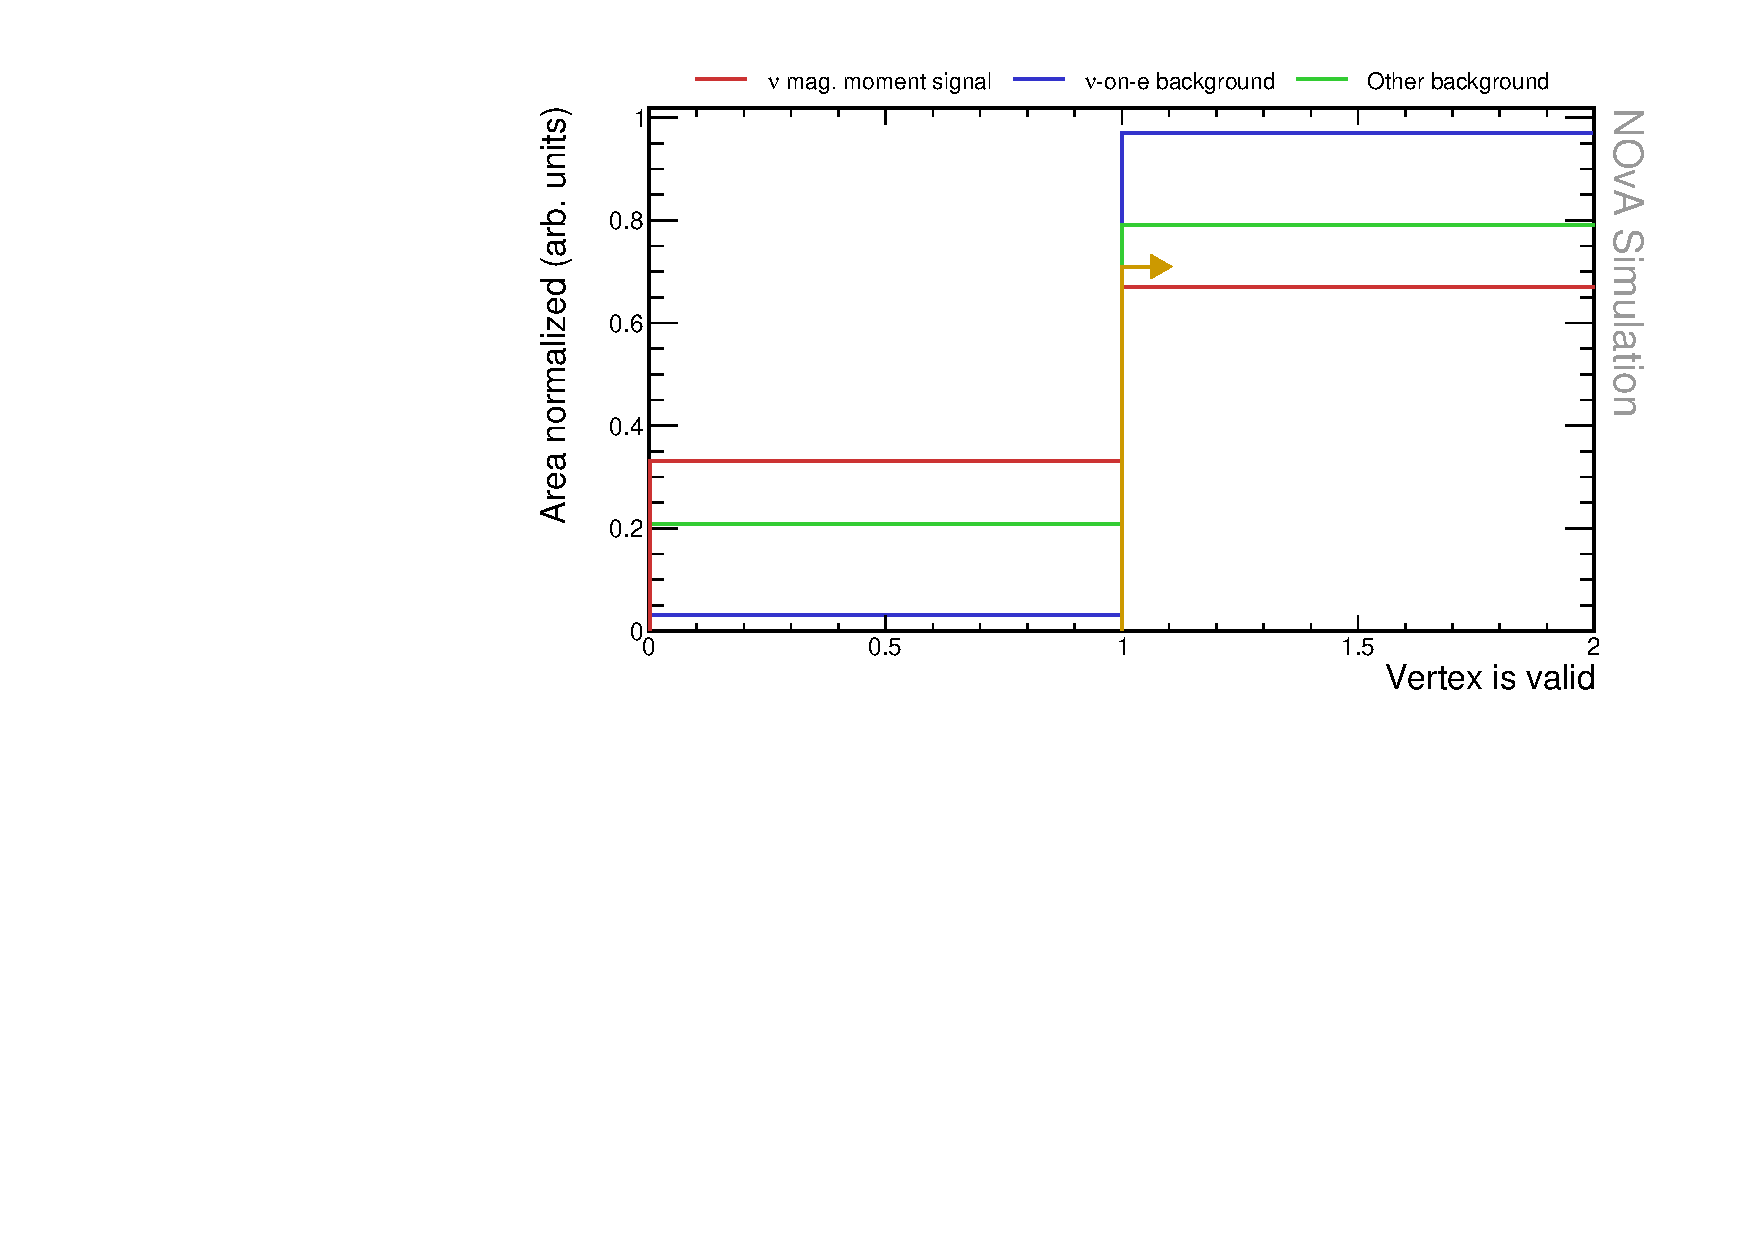
\includegraphics[width=.49\textwidth]{Plots/AnalysisOverview/NoCut_vtxIsValid.pdf}
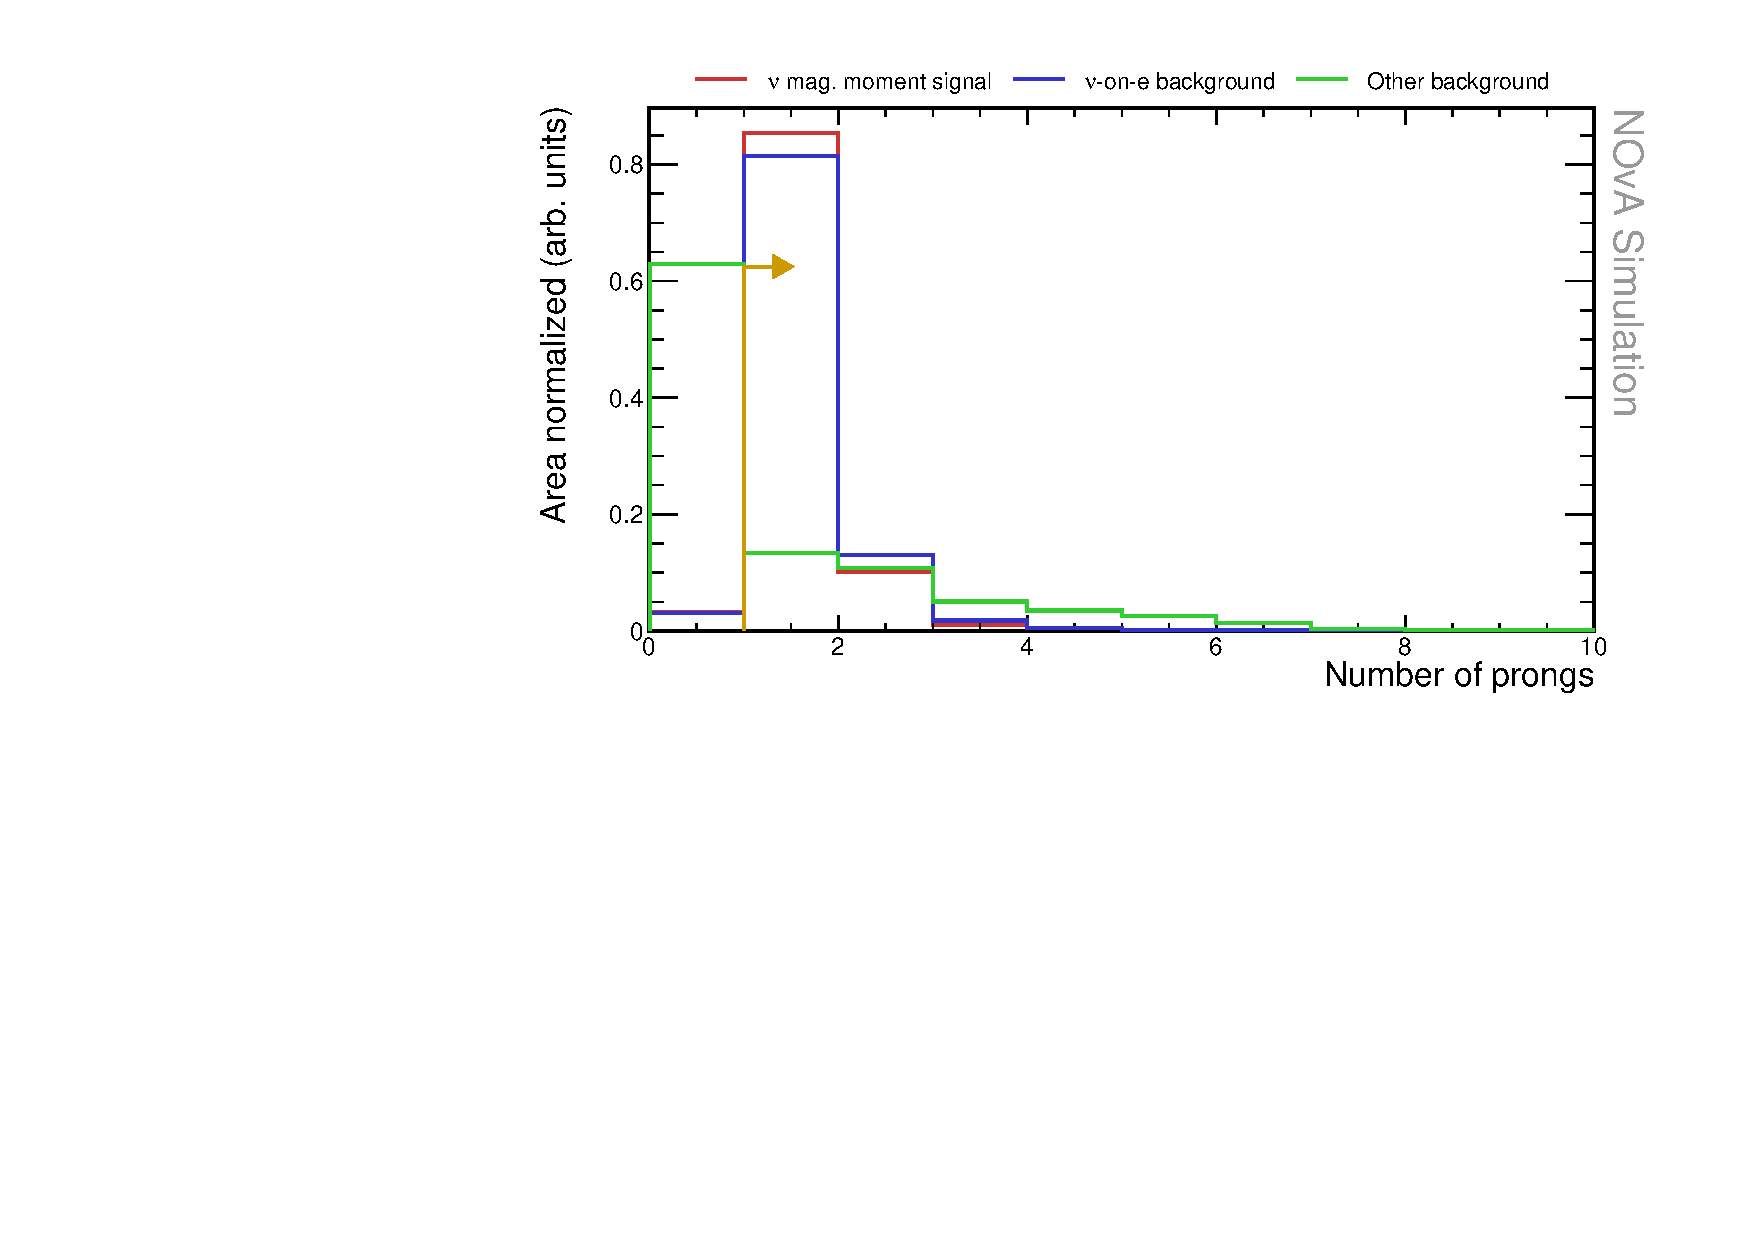
\includegraphics[width=.49\textwidth]{Plots/AnalysisOverview/NoCut_NPng.pdf}
\caption{Relative comparison of signal, $\nu$-on-e background, and other background events for basic pre-selection variables. No cuts were applied to make these plots. Gold lines show the cut values for the shown variables.}
\label{fig:BasicPreSelectionCuts}
\end{figure}

\begin{figure}[hbtp]
\centering
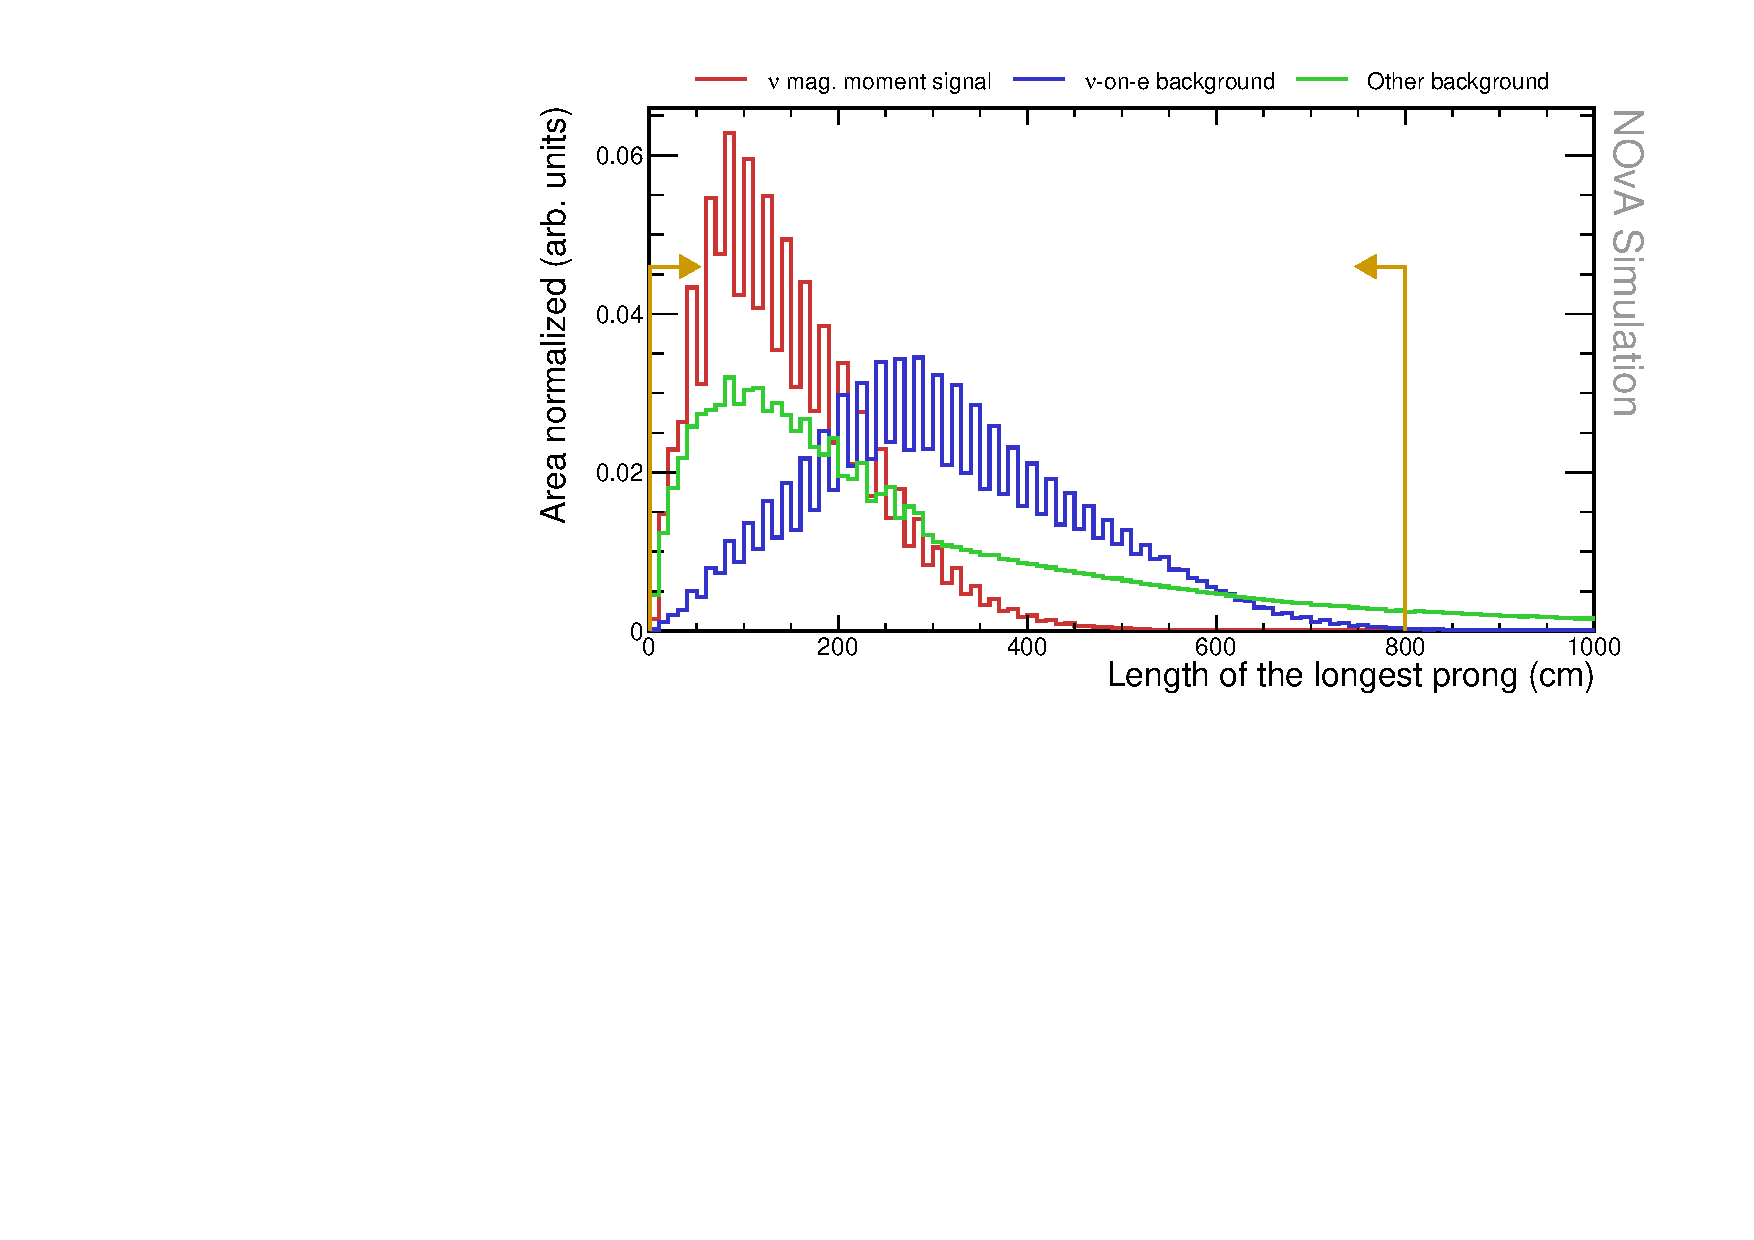
\includegraphics[width=.49\textwidth]{Plots/AnalysisOverview/N1Cut_longestProng.pdf}
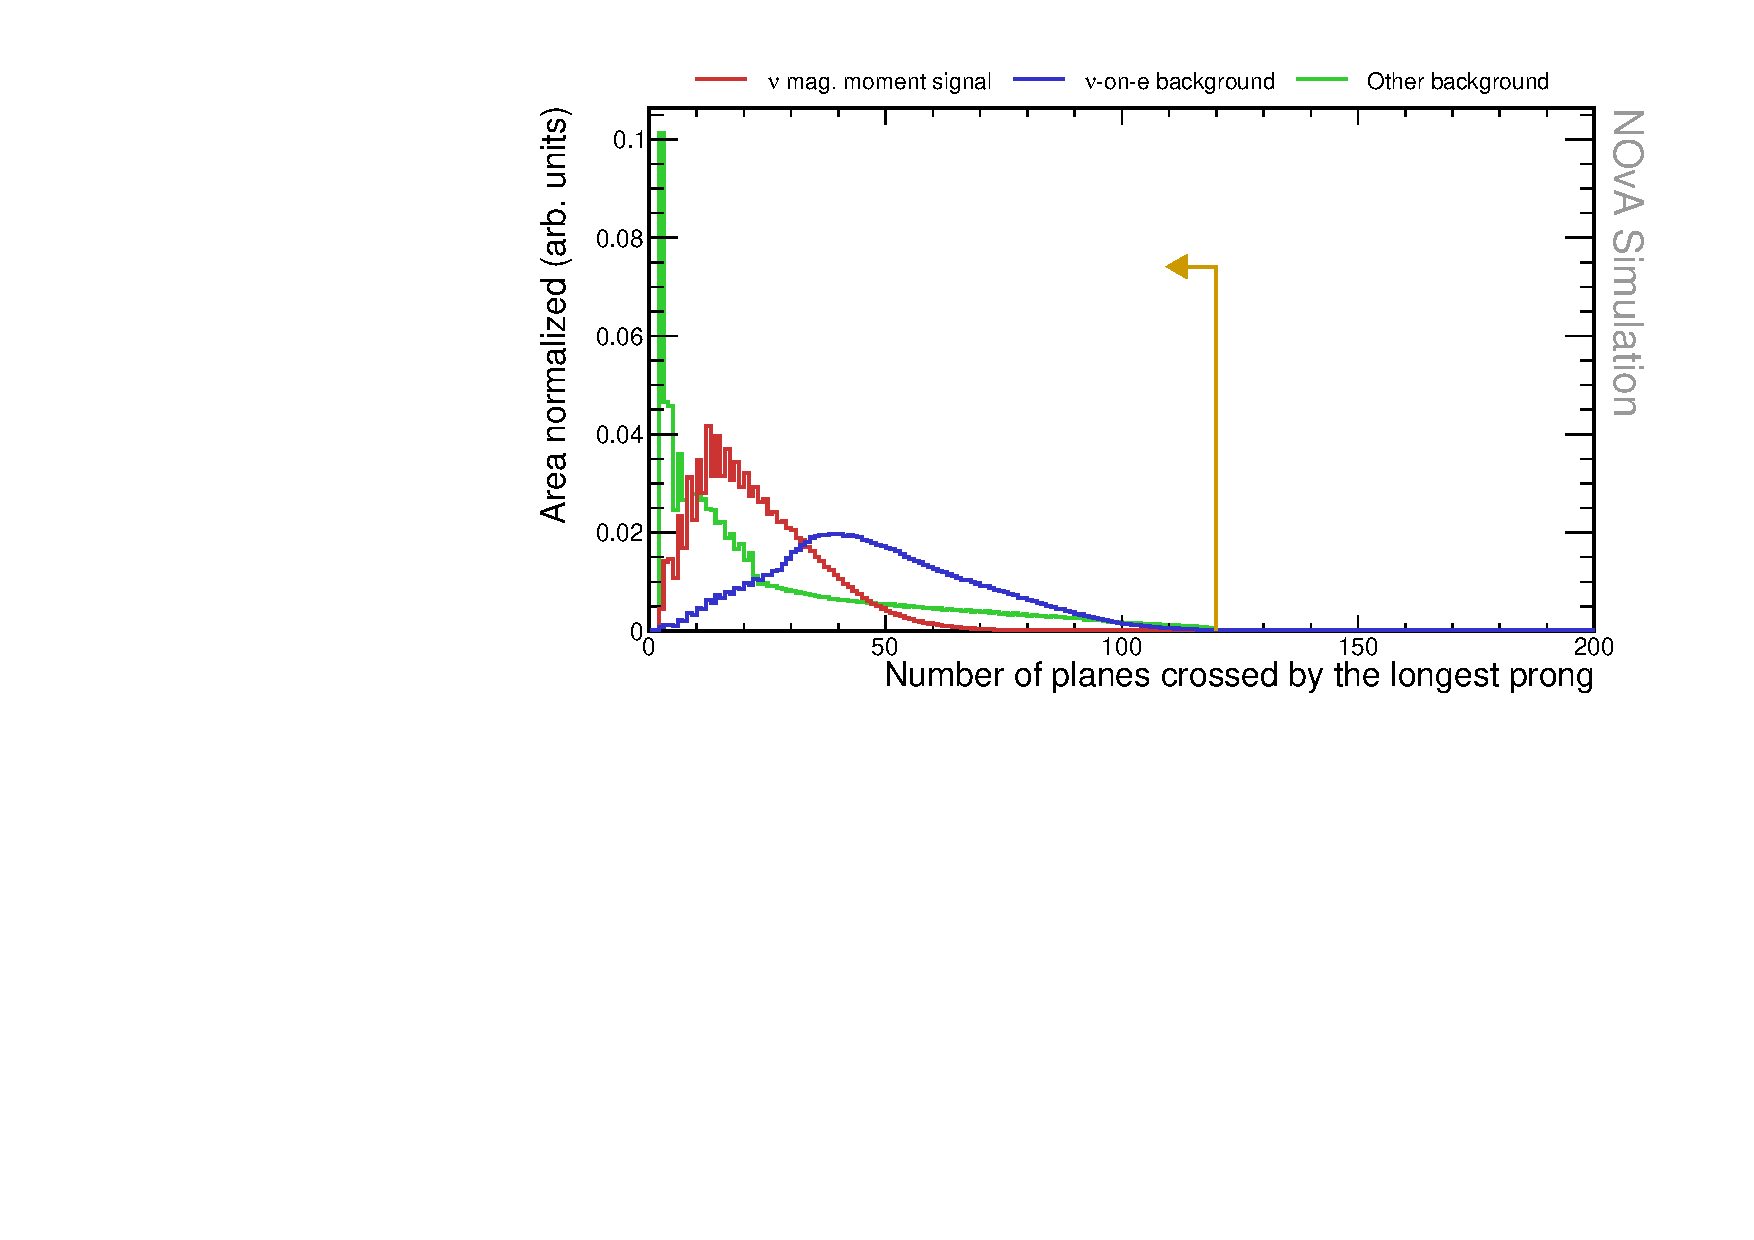
\includegraphics[width=.49\textwidth]{Plots/AnalysisOverview/N1Cut_NPlanes.pdf}
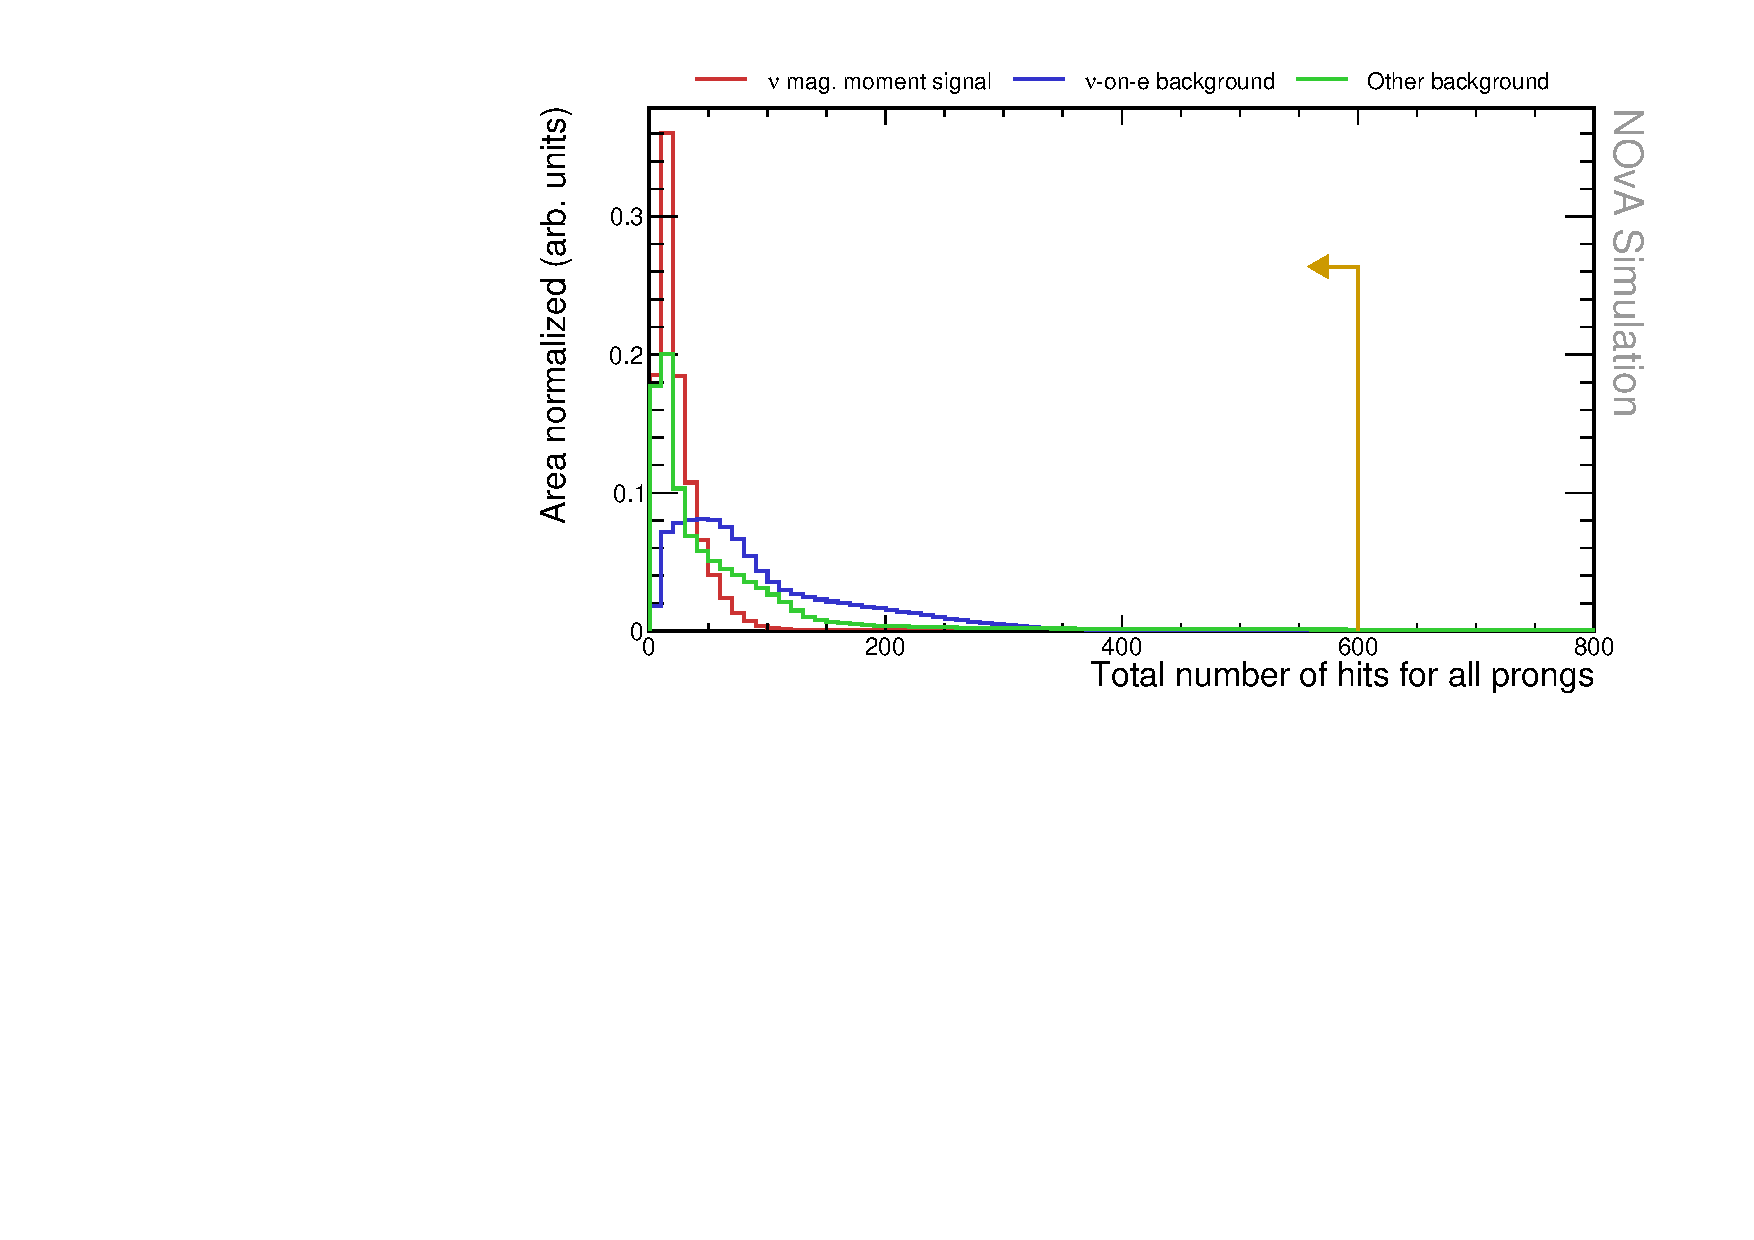
\includegraphics[width=.49\textwidth]{Plots/AnalysisOverview/N1Cut_NHits.pdf}
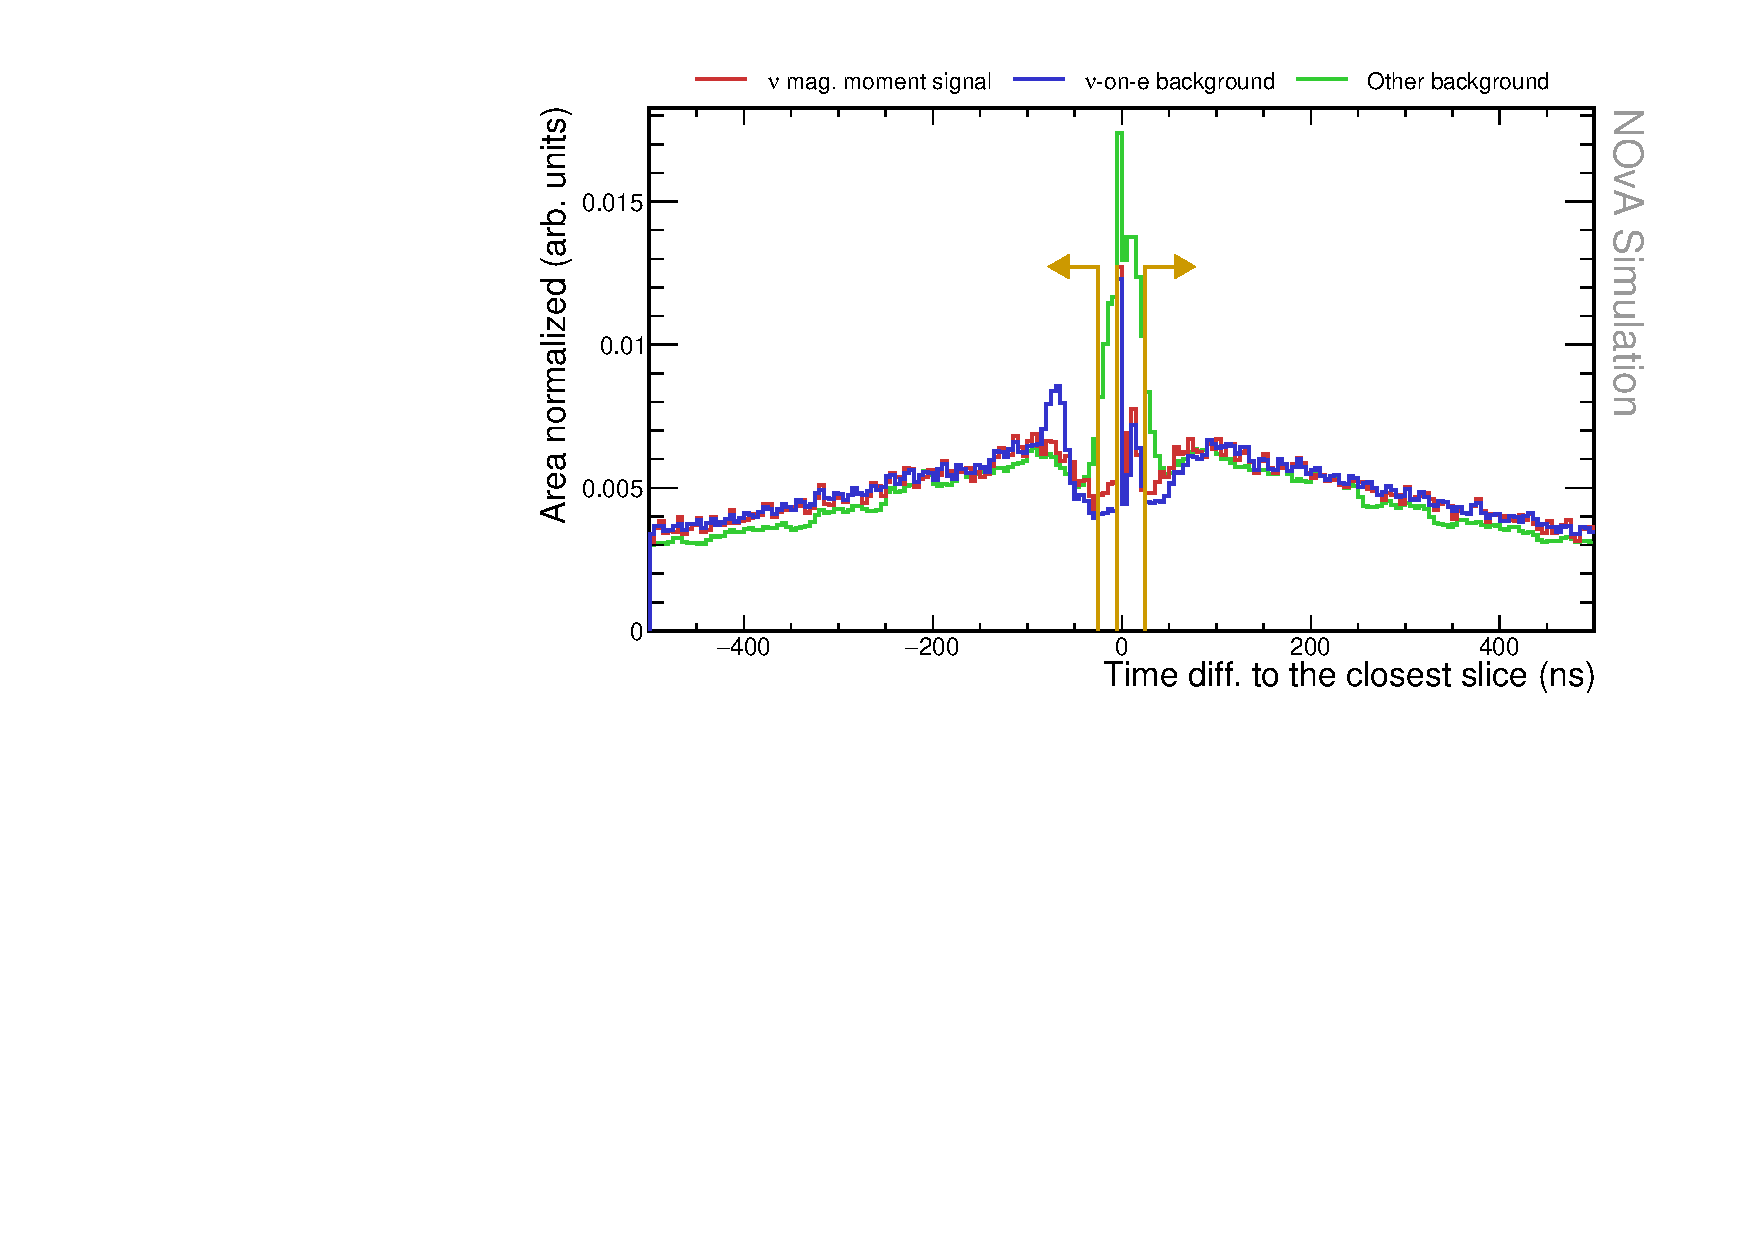
\includegraphics[width=.49\textwidth]{Plots/AnalysisOverview/N1Cut_closestSlice.pdf}
\caption{Relative comparison of signal, $\nu$-on-e background, and other background events for pre-selection variables. Cuts on VtxIsValid and number of prongs were applied to make these plots. Gold lines show the cut values for the shown variables.}
\label{fig:PreSelectionCuts}
\end{figure}

%\todo{Add the DeCAF cuts description here - might describe them already when introducing the decaf samples, not sure yet}

\subsubsection*{Fiducial and containment cuts}

\todo{Describe what does the fiducial cut do}
We require that the reconstructed vertex is contained within the following volume: $-185<\textsf{Vtx}_X<175,-175<\textsf{Vtx}_Y<175, 95<\textsf{Vtx}_Z<1095\ \unit{cm}$.

\begin{figure}[hbtp]
\centering
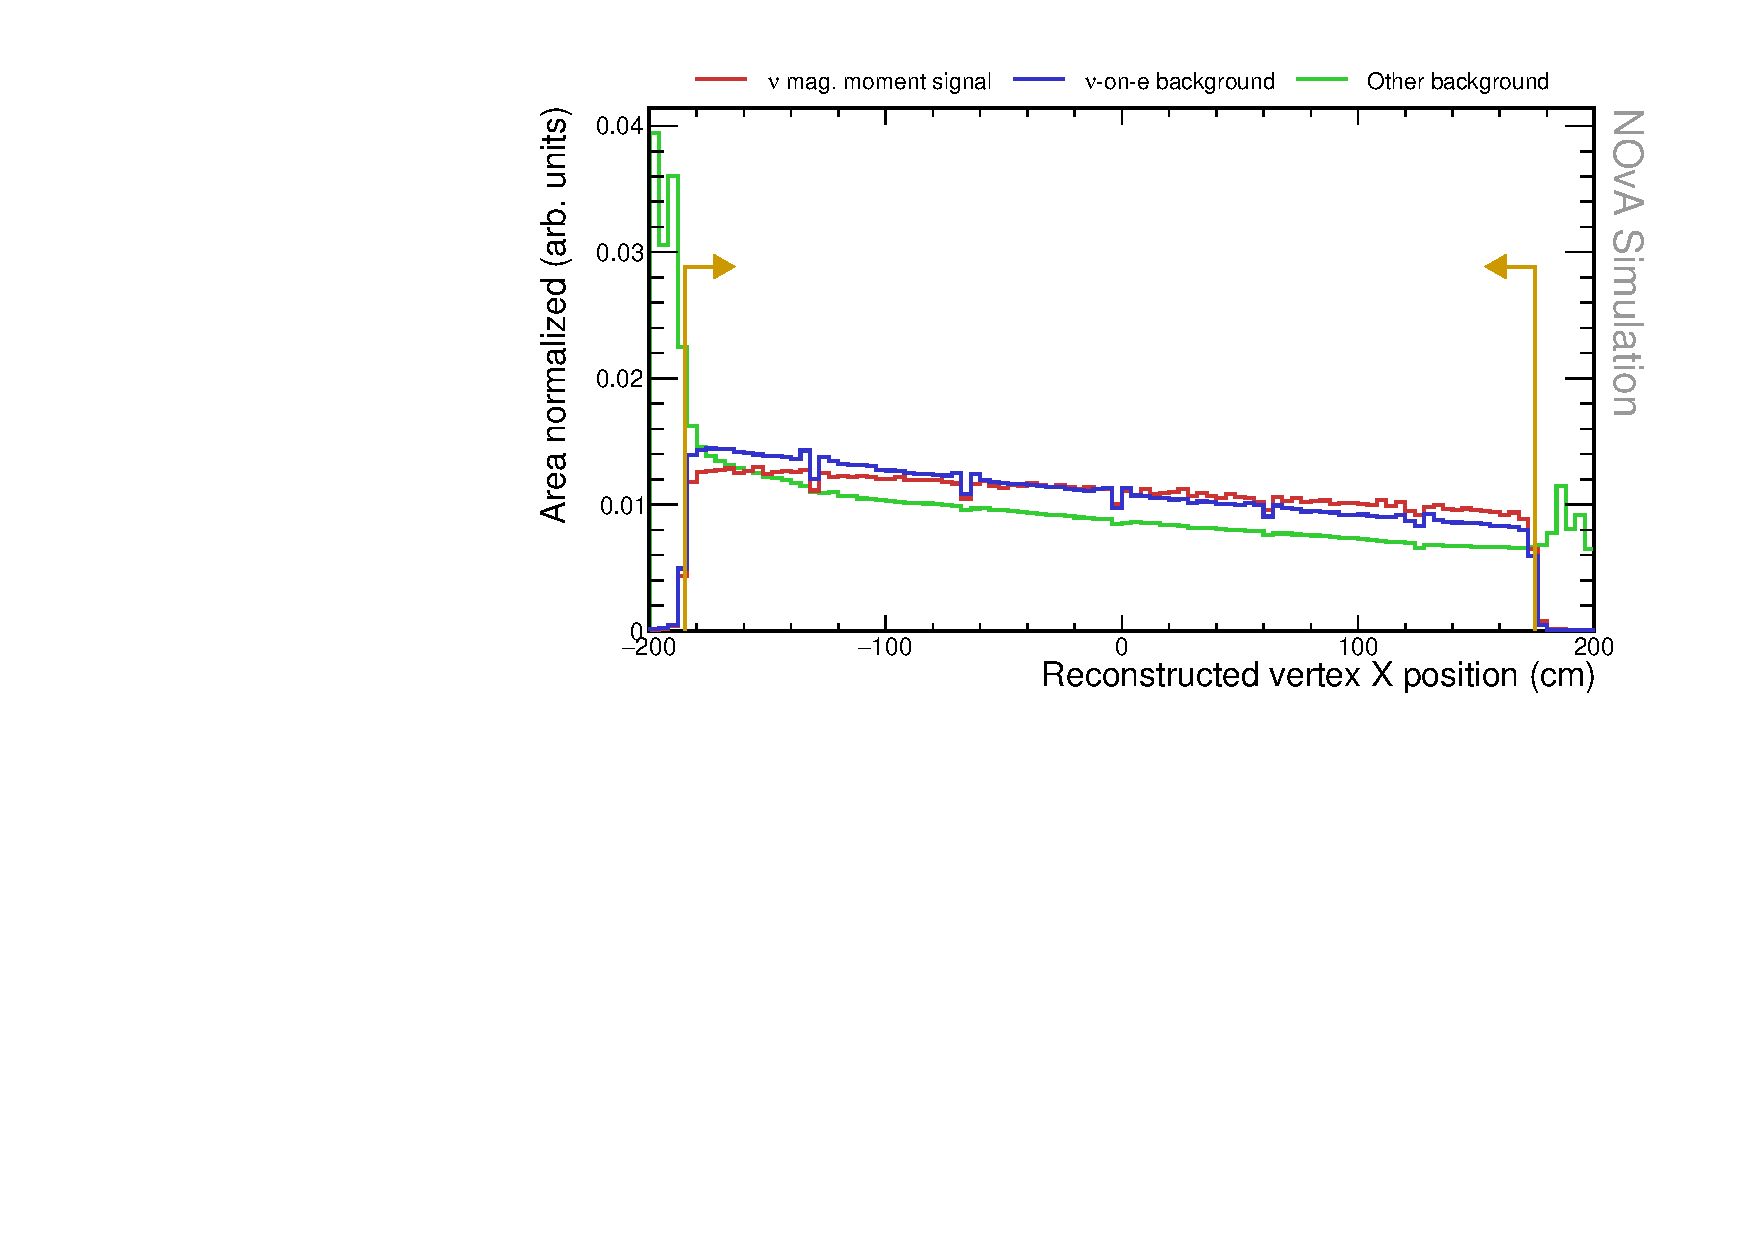
\includegraphics[width=.49\textwidth]{Plots/AnalysisOverview/NoCut_vtxX.pdf}
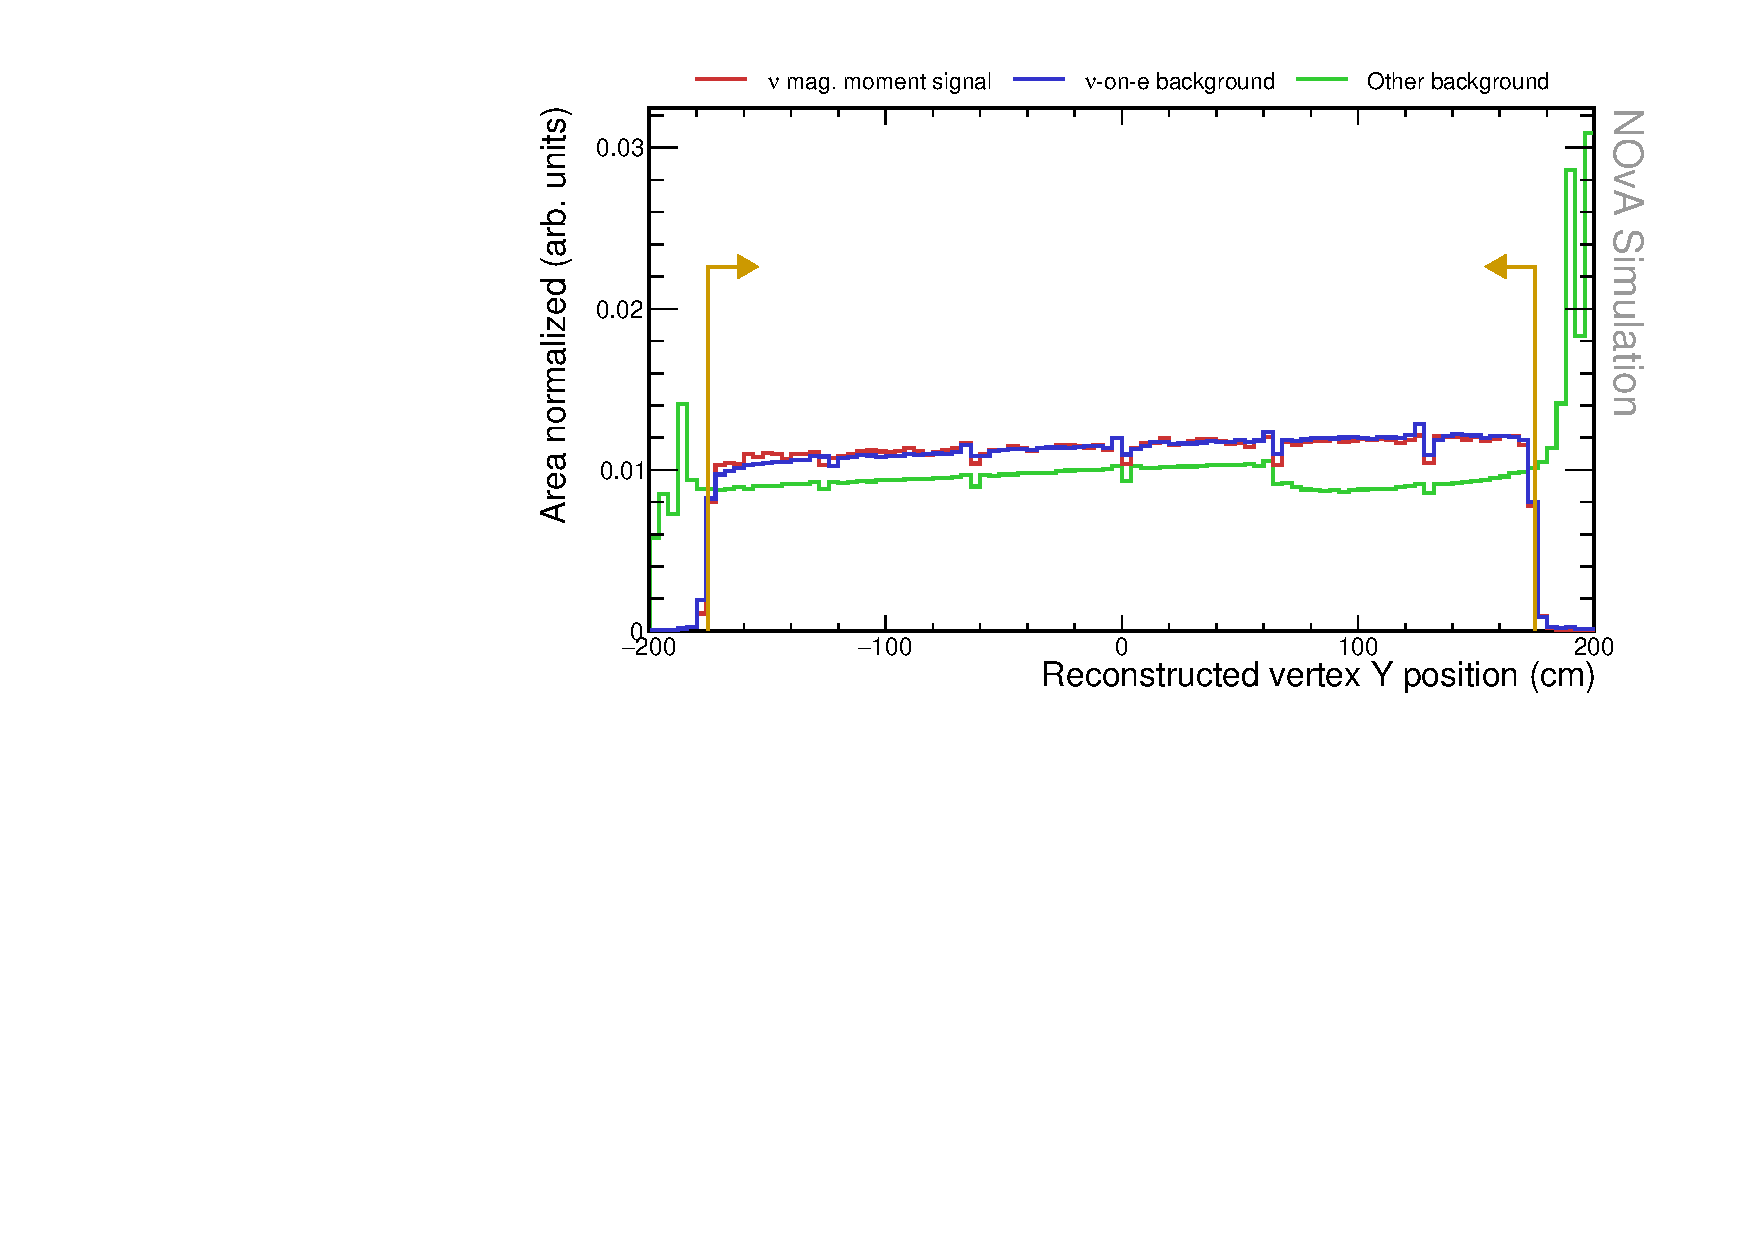
\includegraphics[width=.49\textwidth]{Plots/AnalysisOverview/NoCut_vtxY.pdf}
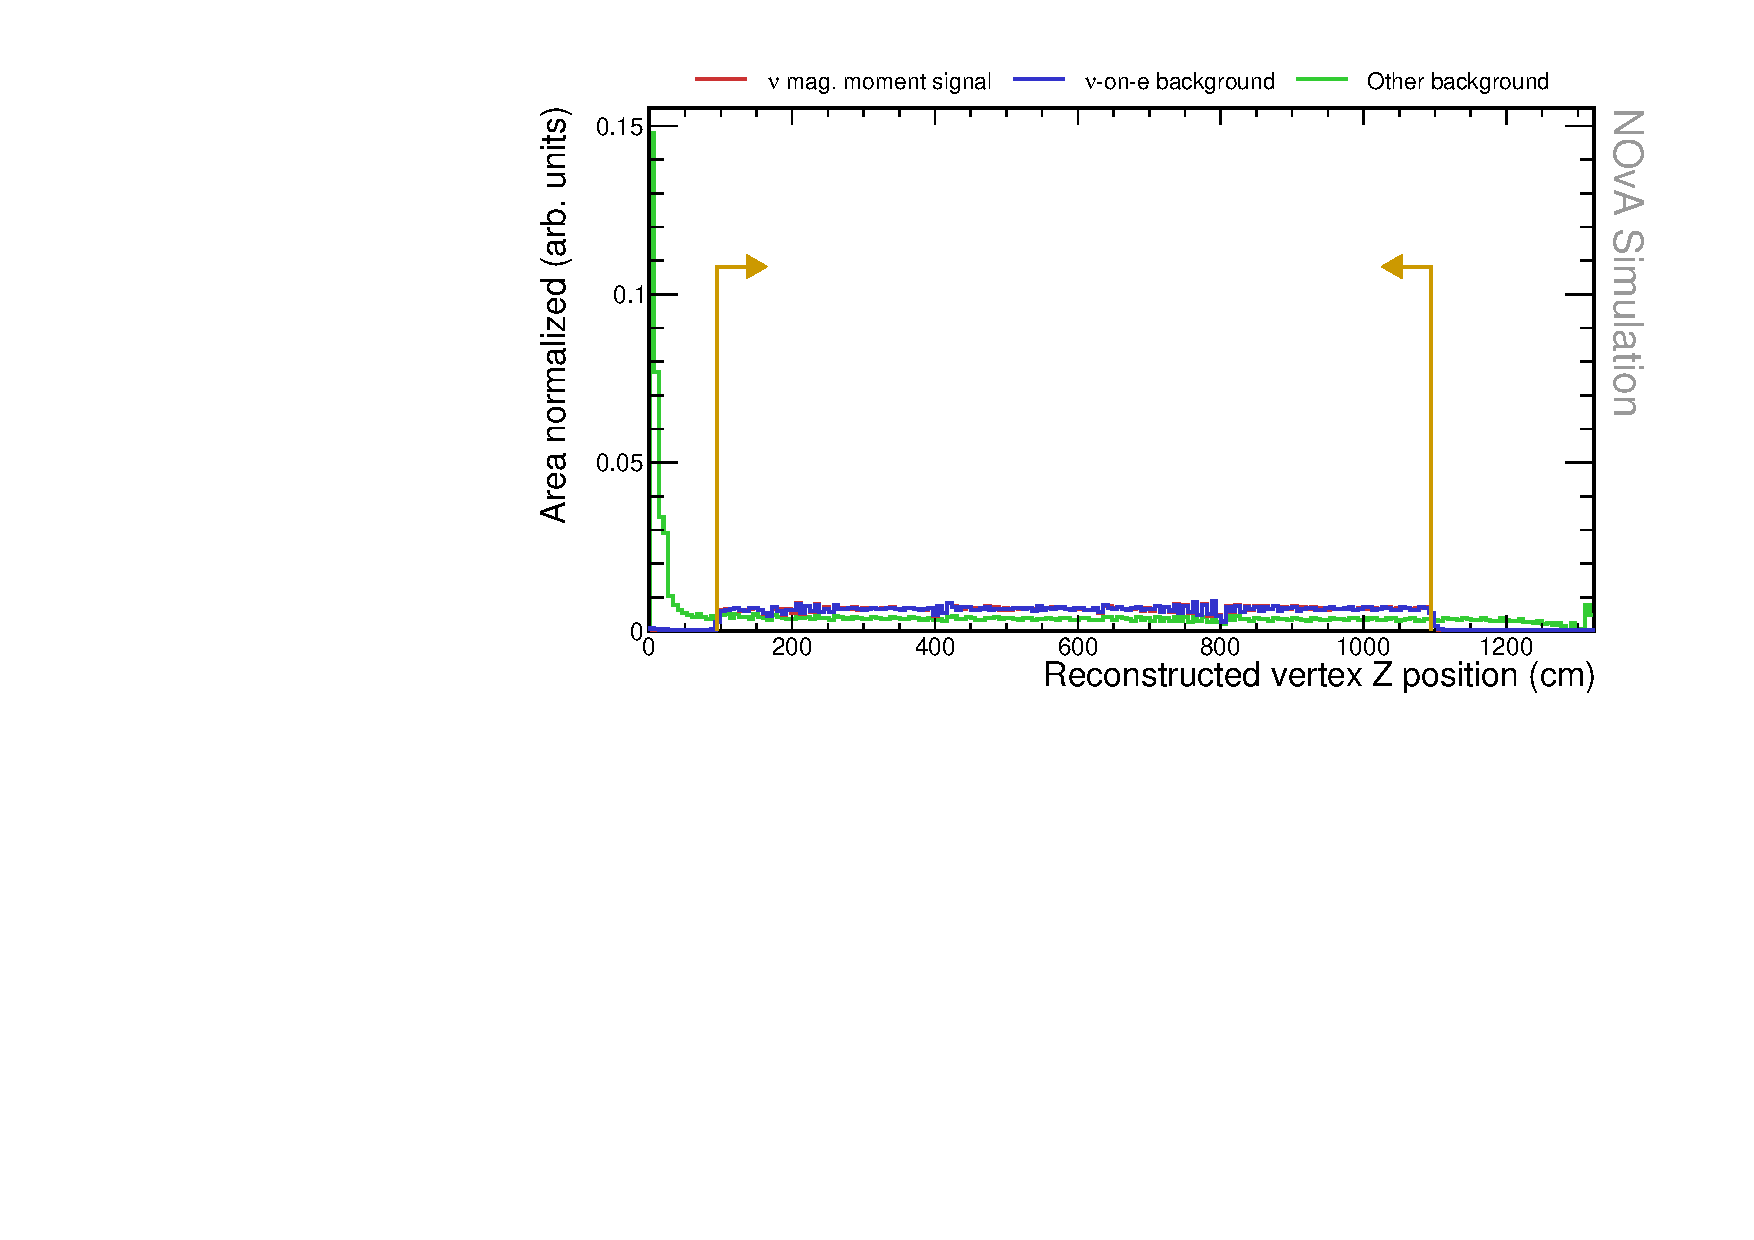
\includegraphics[width=.49\textwidth]{Plots/AnalysisOverview/NoCut_vtxZ.pdf}
\caption{Relative comparison of signal, $\nu$-on-e background, and other background events for the reconstructed vertex. No cuts were applied to make these plots. Gold lines show the cut values that create the fiducial volume.}
\label{fig:FiducialCut}
\end{figure}

To ensure all the energy is contained within the detector and to remove events originating outside of the detector (rock muons), we require that the extreme positions of hits for all prongs in the slice are within the following volume: $-190<\textsf{min}_X, \textsf{max}_X<180, -180<\textsf{min}_Y, \textsf{max}_Y<190, 105<\textsf{min}_Z, \textsf{max}_Z<1275\ \unit{cm}$.

\begin{figure}[hbtp]
\centering
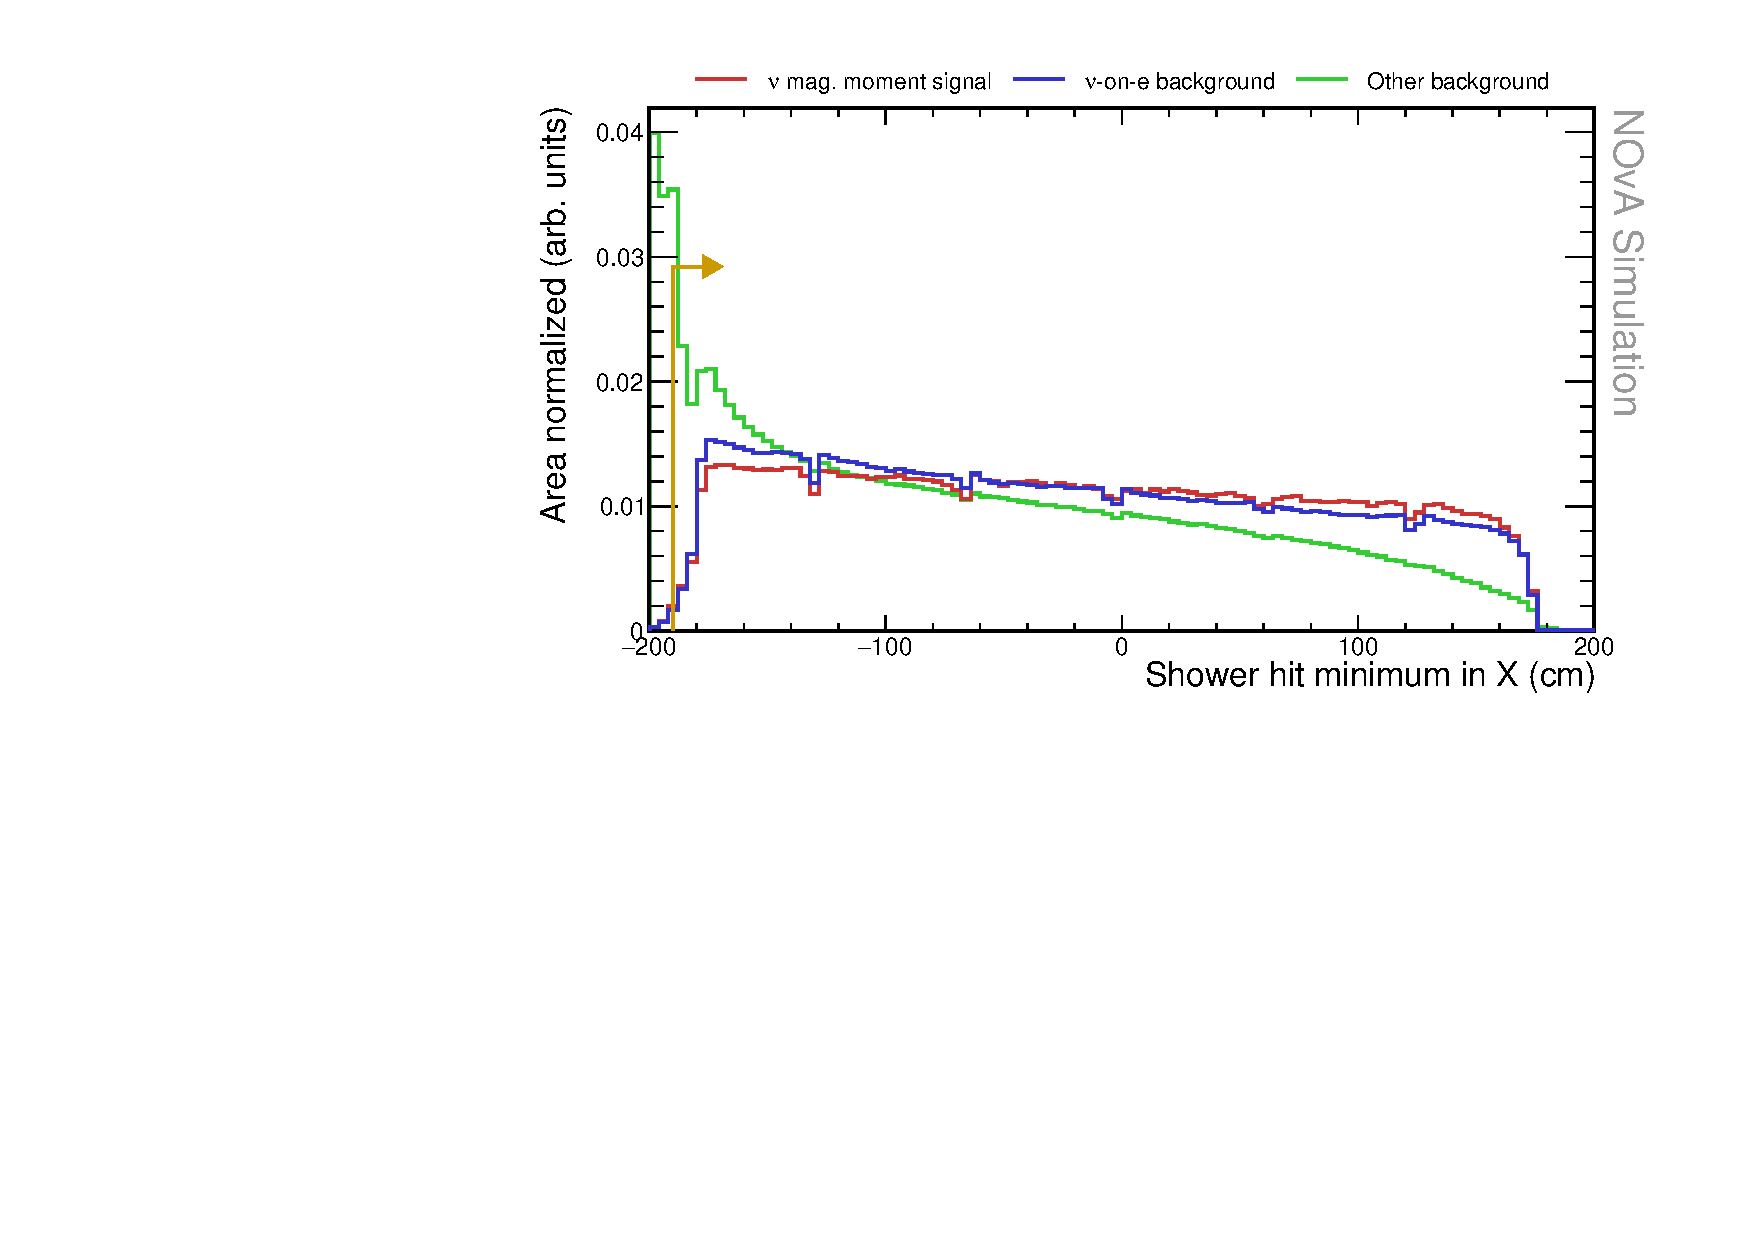
\includegraphics[width=.49\textwidth]{Plots/AnalysisOverview/N1Cut_minX.pdf}
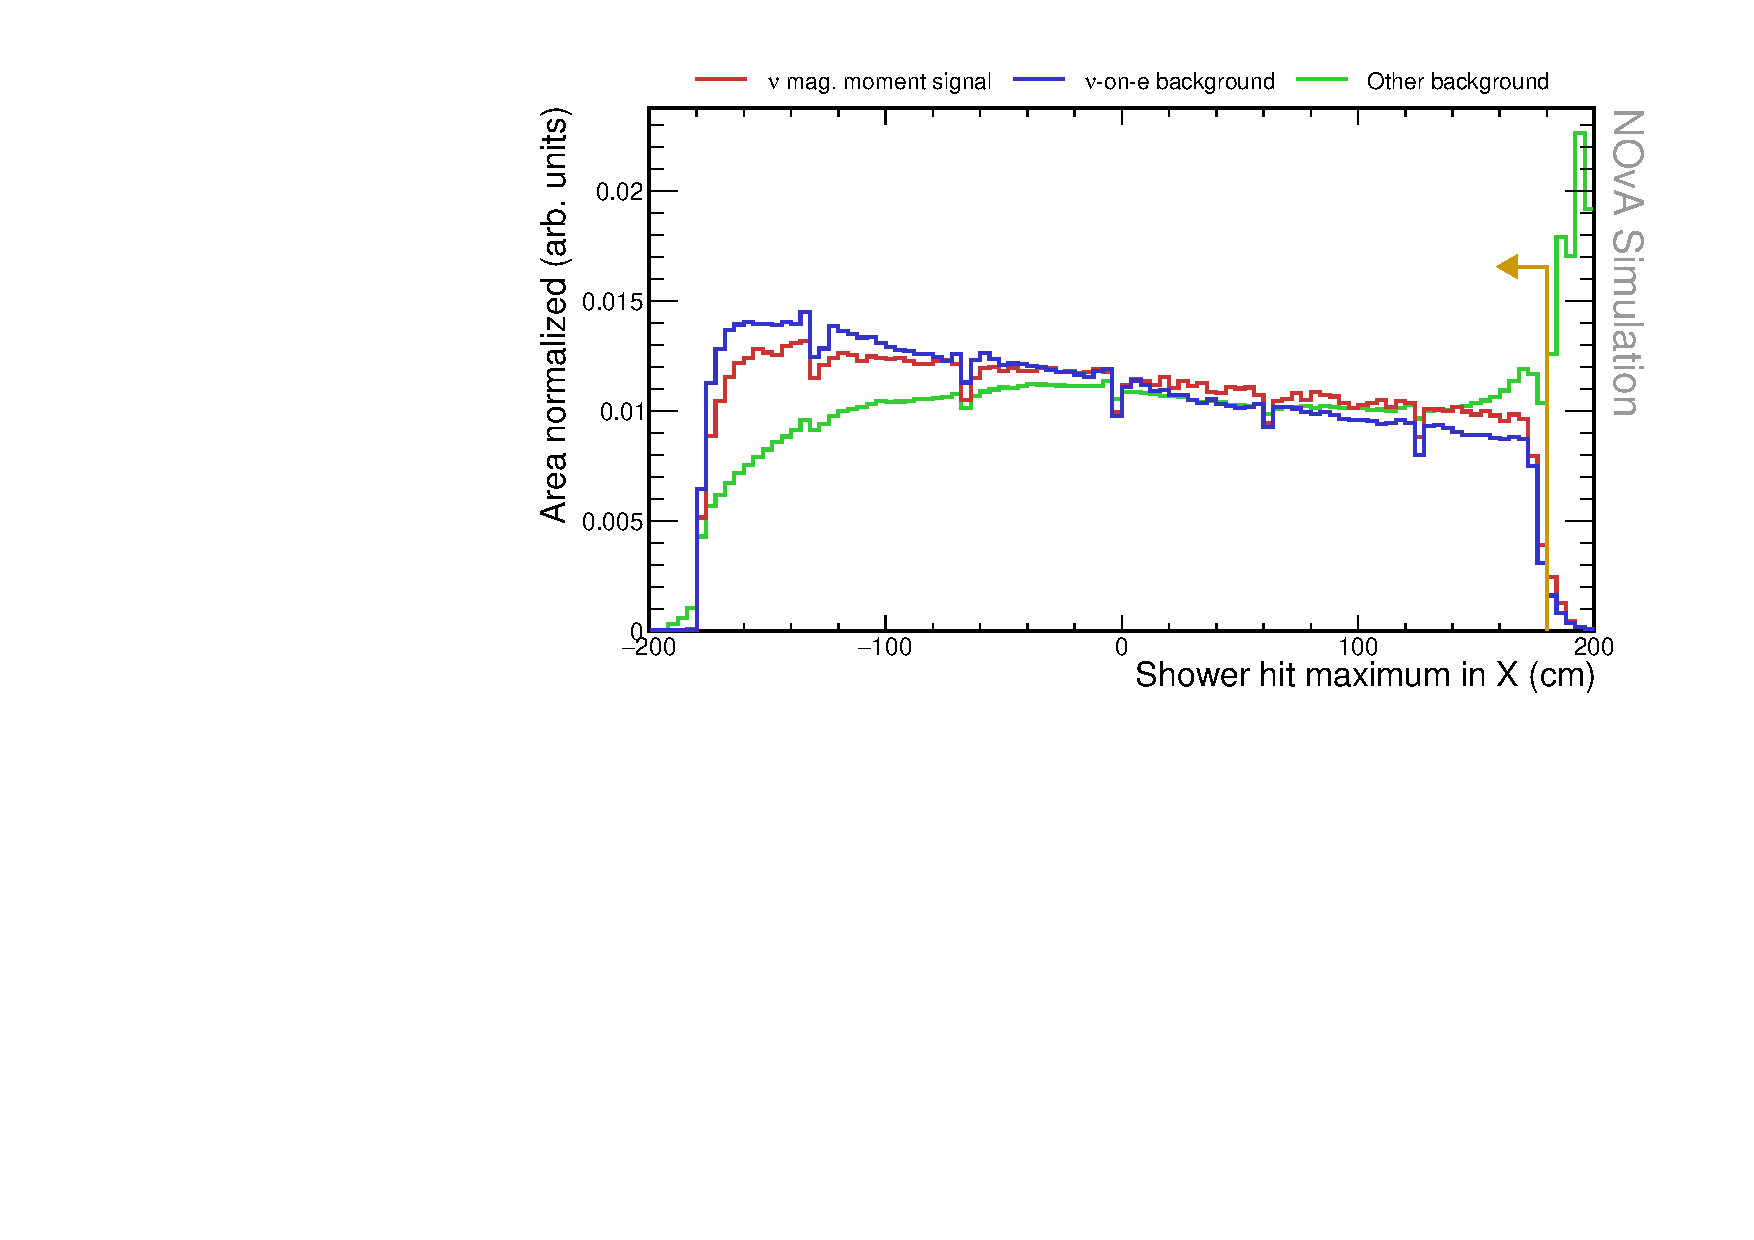
\includegraphics[width=.49\textwidth]{Plots/AnalysisOverview/N1Cut_maxX.pdf}
\caption{Relative comparison of signal, $\nu$-on-e background, and other background events for the minimum and maximum position of the reconstructed shower along the X axis. Pre-selection and fiducial cuts were applied to make these plots. Gold lines show the values of the containment cuts.}
\label{fig:ContainmentCutsX}
\end{figure}

\begin{figure}[hbtp]
\centering
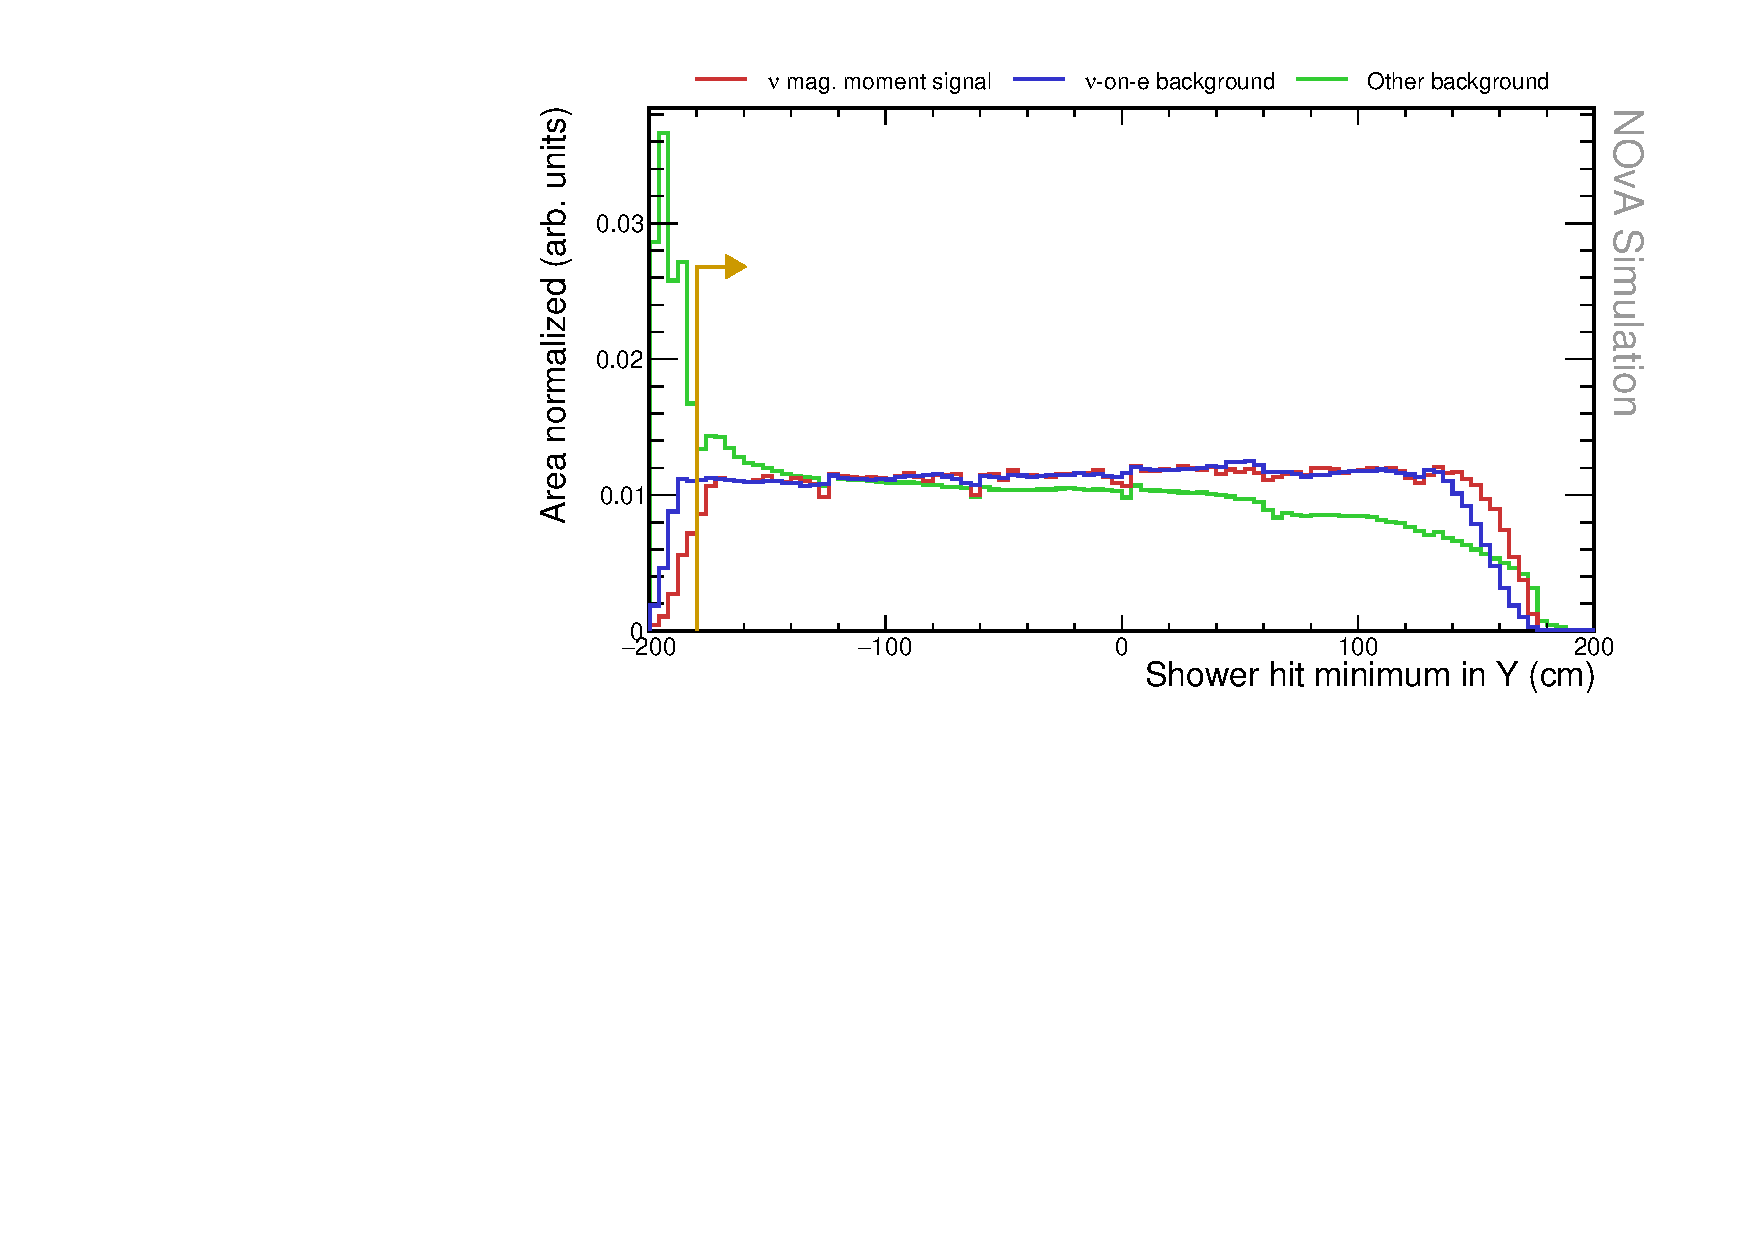
\includegraphics[width=.49\textwidth]{Plots/AnalysisOverview/N1Cut_minY.pdf}
\includegraphics[width=.49\textwidth]{Plots/AnalysisOverview/N1Cut_maxY.pdf}
\caption{Relative comparison of signal, $\nu$-on-e background, and other background events for the minimum and maximum position of the reconstructed shower along the Y axis. Pre-selection and fiducial cuts were applied to make these plots. Gold lines show the values of the containment cuts.}
\label{fig:ContainmentCutsY}
\end{figure}

\begin{figure}[hbtp]
\centering
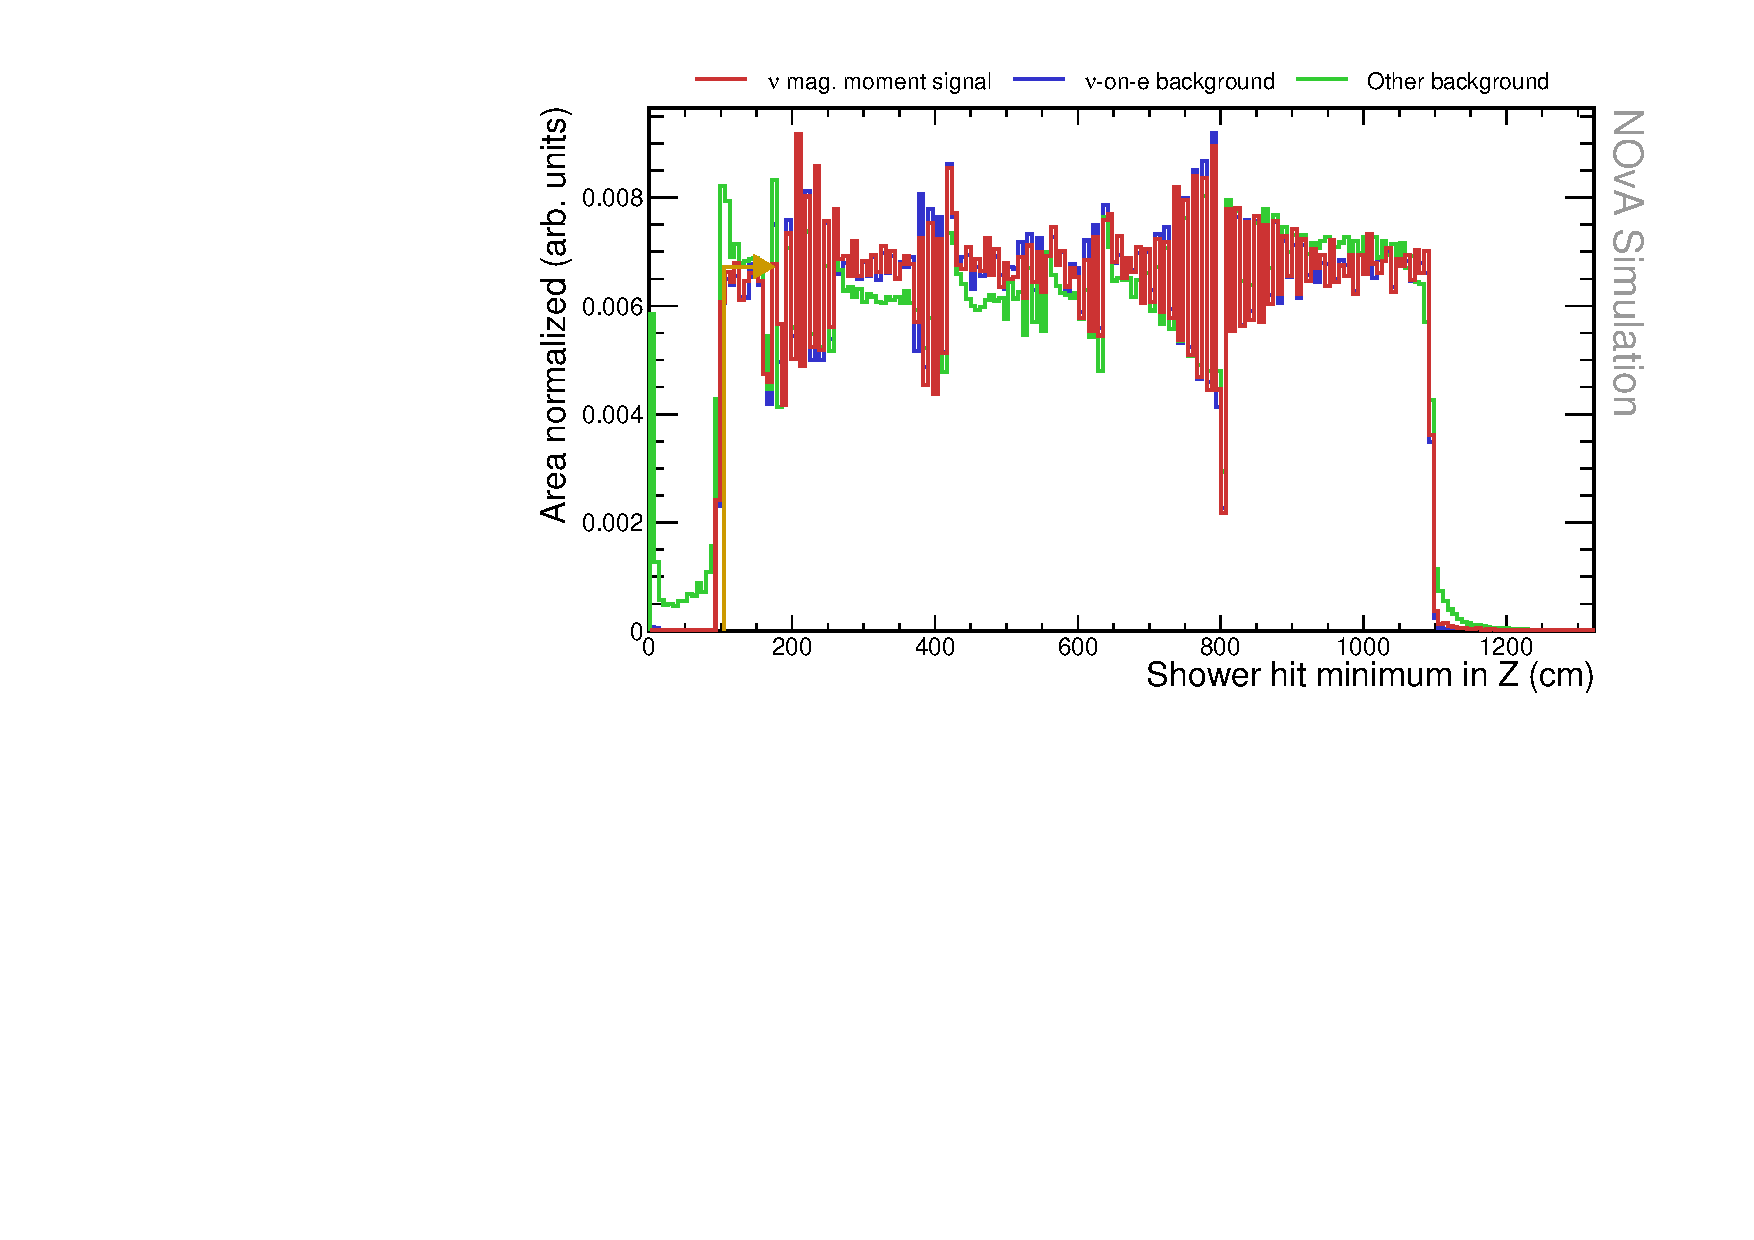
\includegraphics[width=.49\textwidth]{Plots/AnalysisOverview/N1Cut_minZ.pdf}
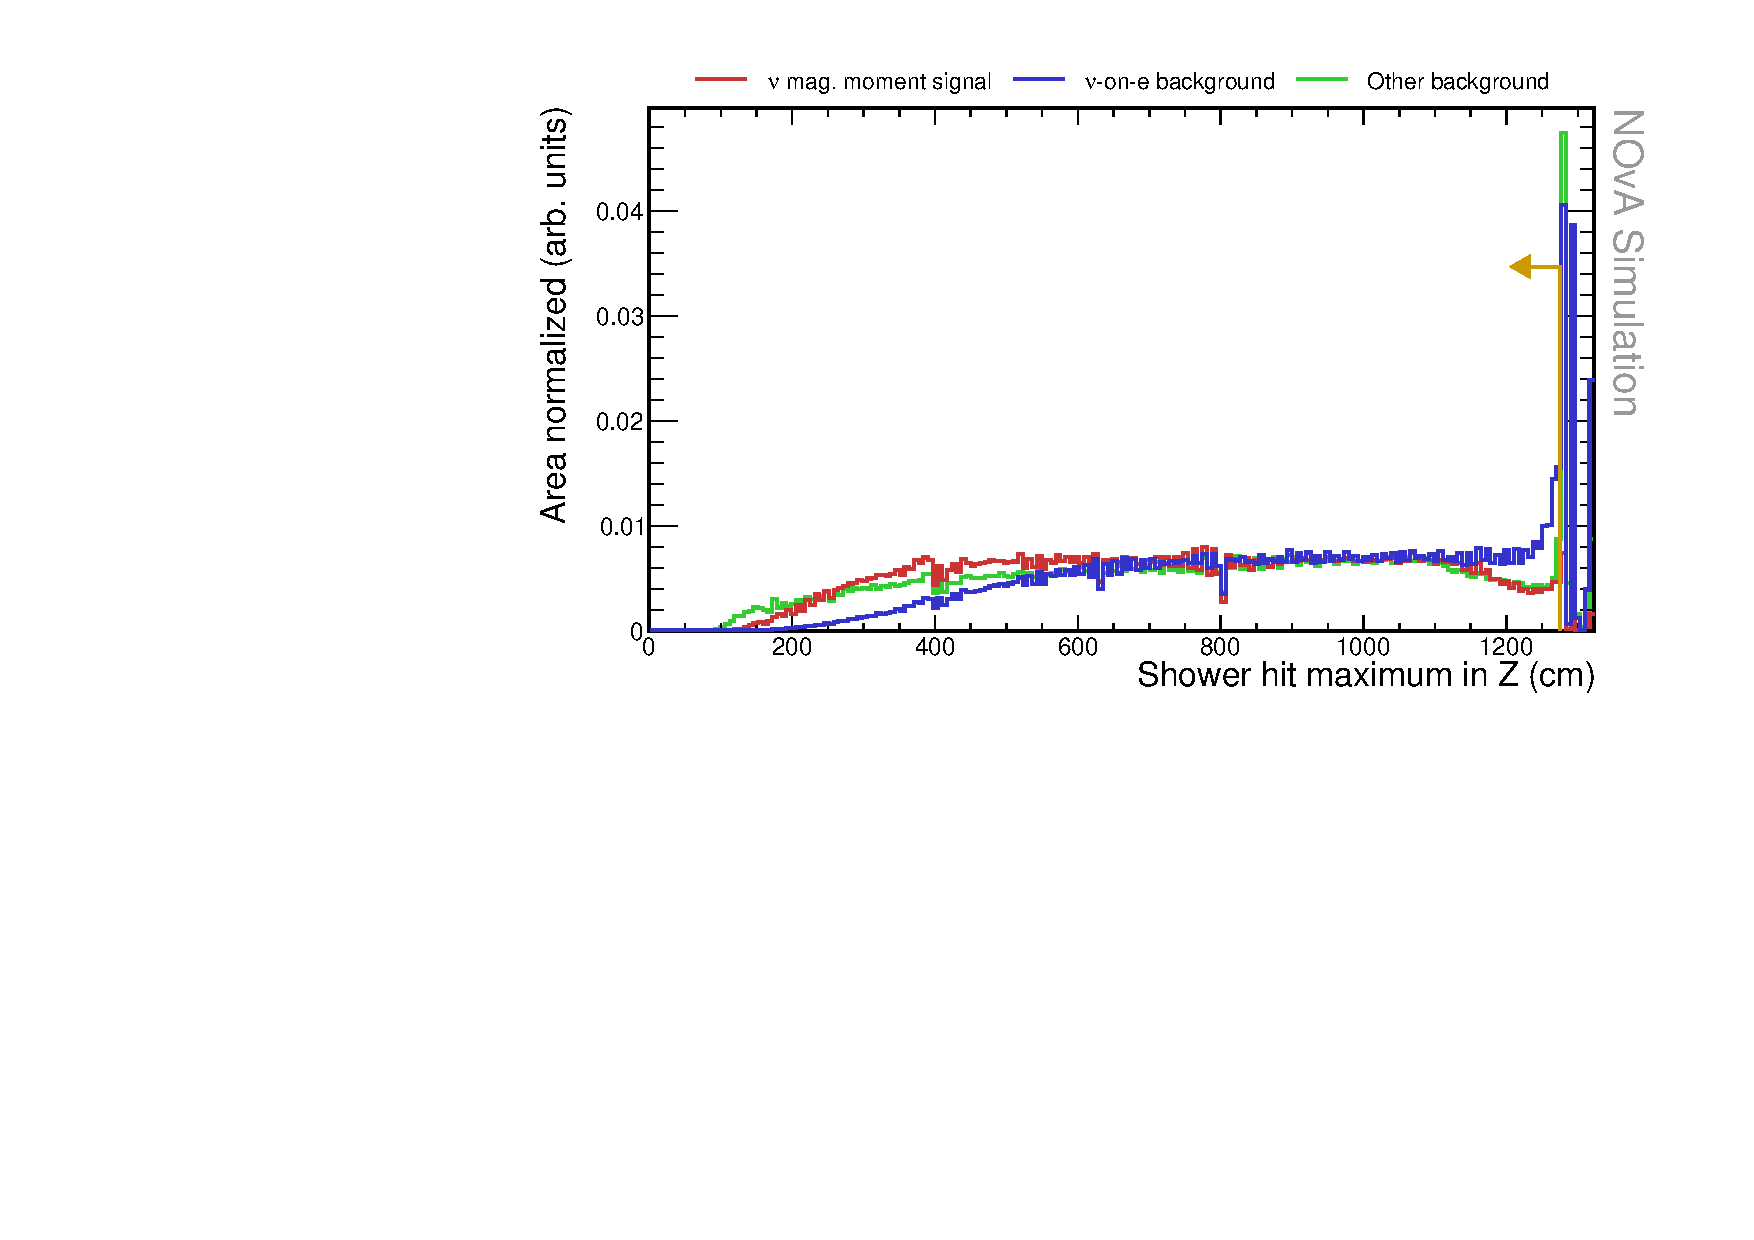
\includegraphics[width=.49\textwidth]{Plots/AnalysisOverview/N1Cut_maxZ.pdf}
\caption{Relative comparison of signal, $\nu$-on-e background, and other background events for the minimum and maximum position of the reconstructed shower along the Z axis. Pre-selection and fiducial cuts were applied to make these plots. Gold lines show the values of the containment cuts.}
\label{fig:ContainmentCutsZ}
\end{figure}

\subsubsection*{Single particle requirement}

To selection events with a single particle we require that the fraction of energy contained in the most energetic shower is $>0.8$, that the summed energy of all cells (above threshold and within $\pm8$ planes from the vertex) outside of the most energetic shower is $<0.02\ \unit{GeV}$, and that the distance between the vertex and the start of the primary shower is $<20\ \unit{cm}$.

\begin{figure}[hbtp]
\centering
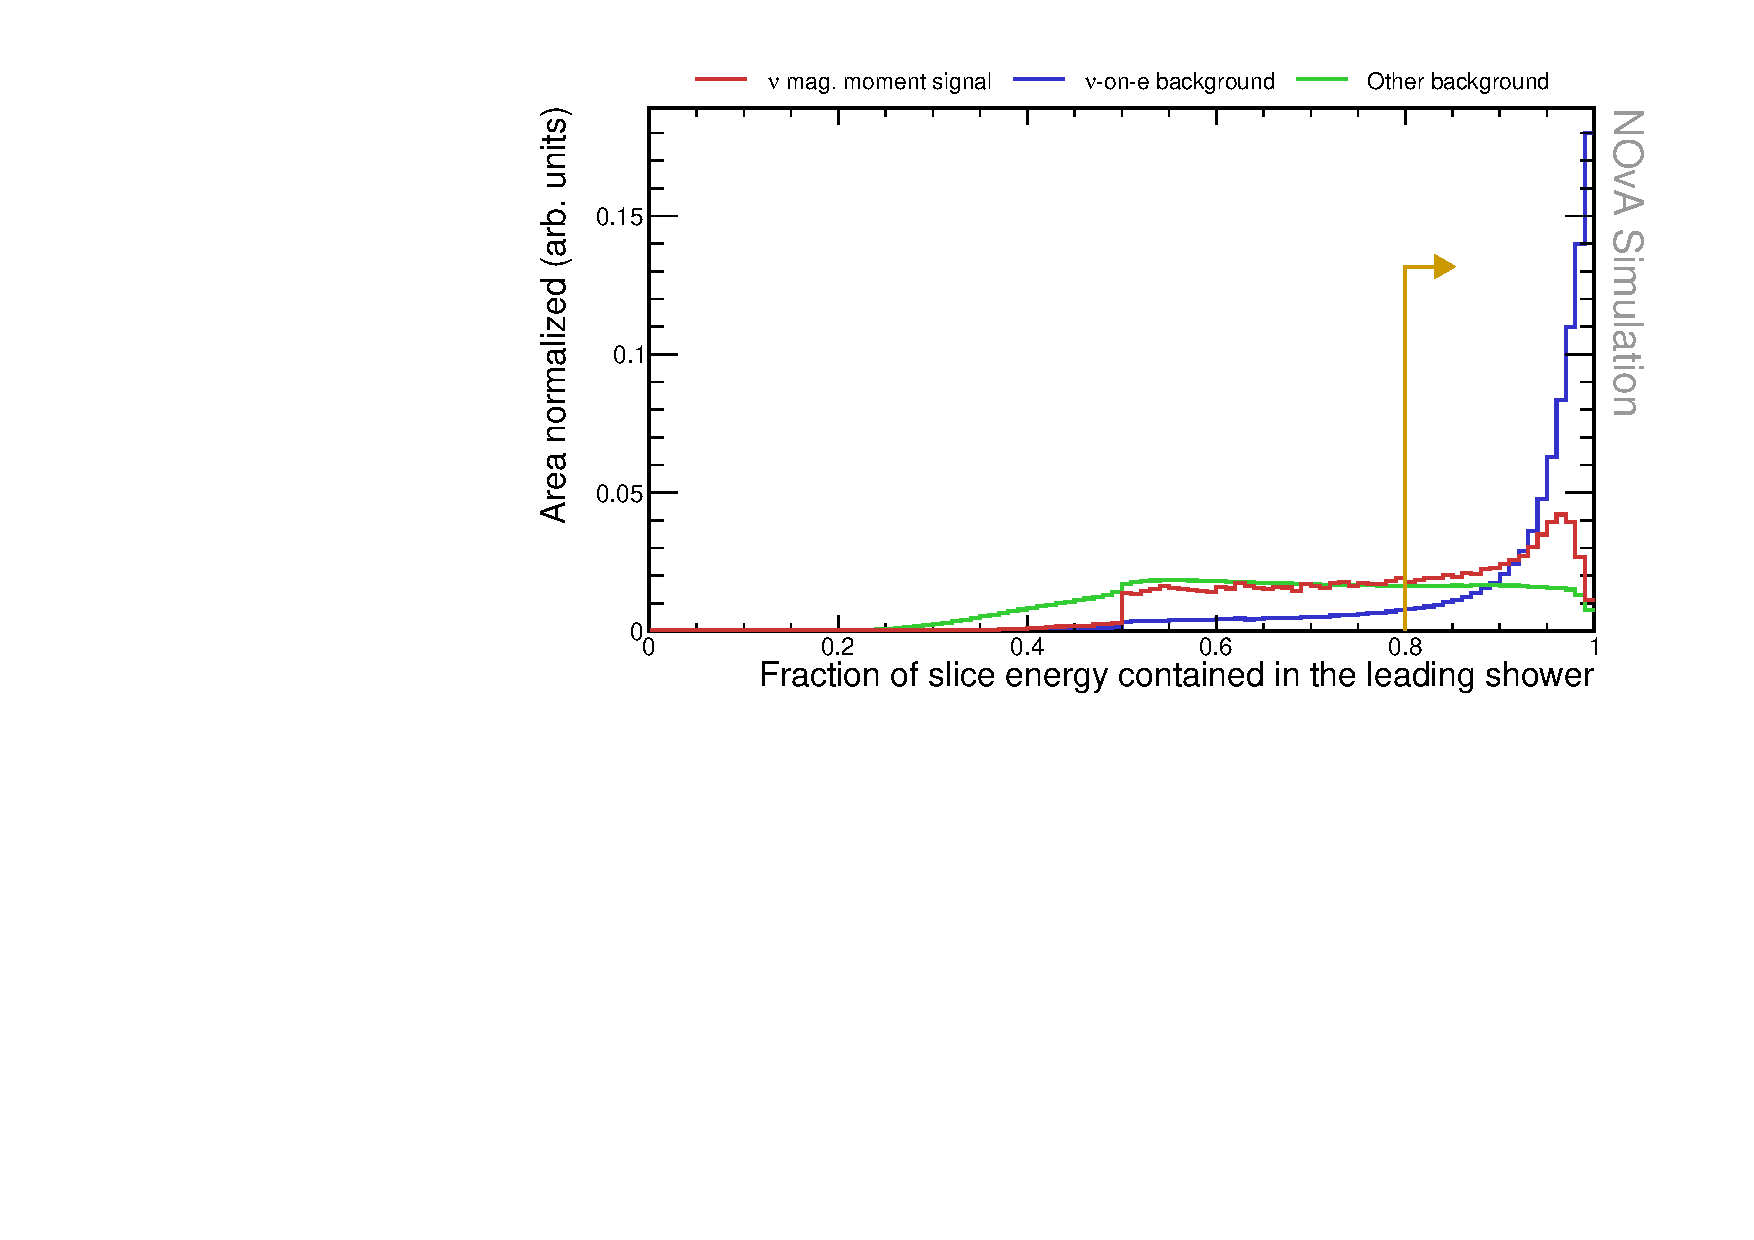
\includegraphics[width=.49\textwidth]{Plots/AnalysisOverview/N1Cut_showerEFrac.pdf}
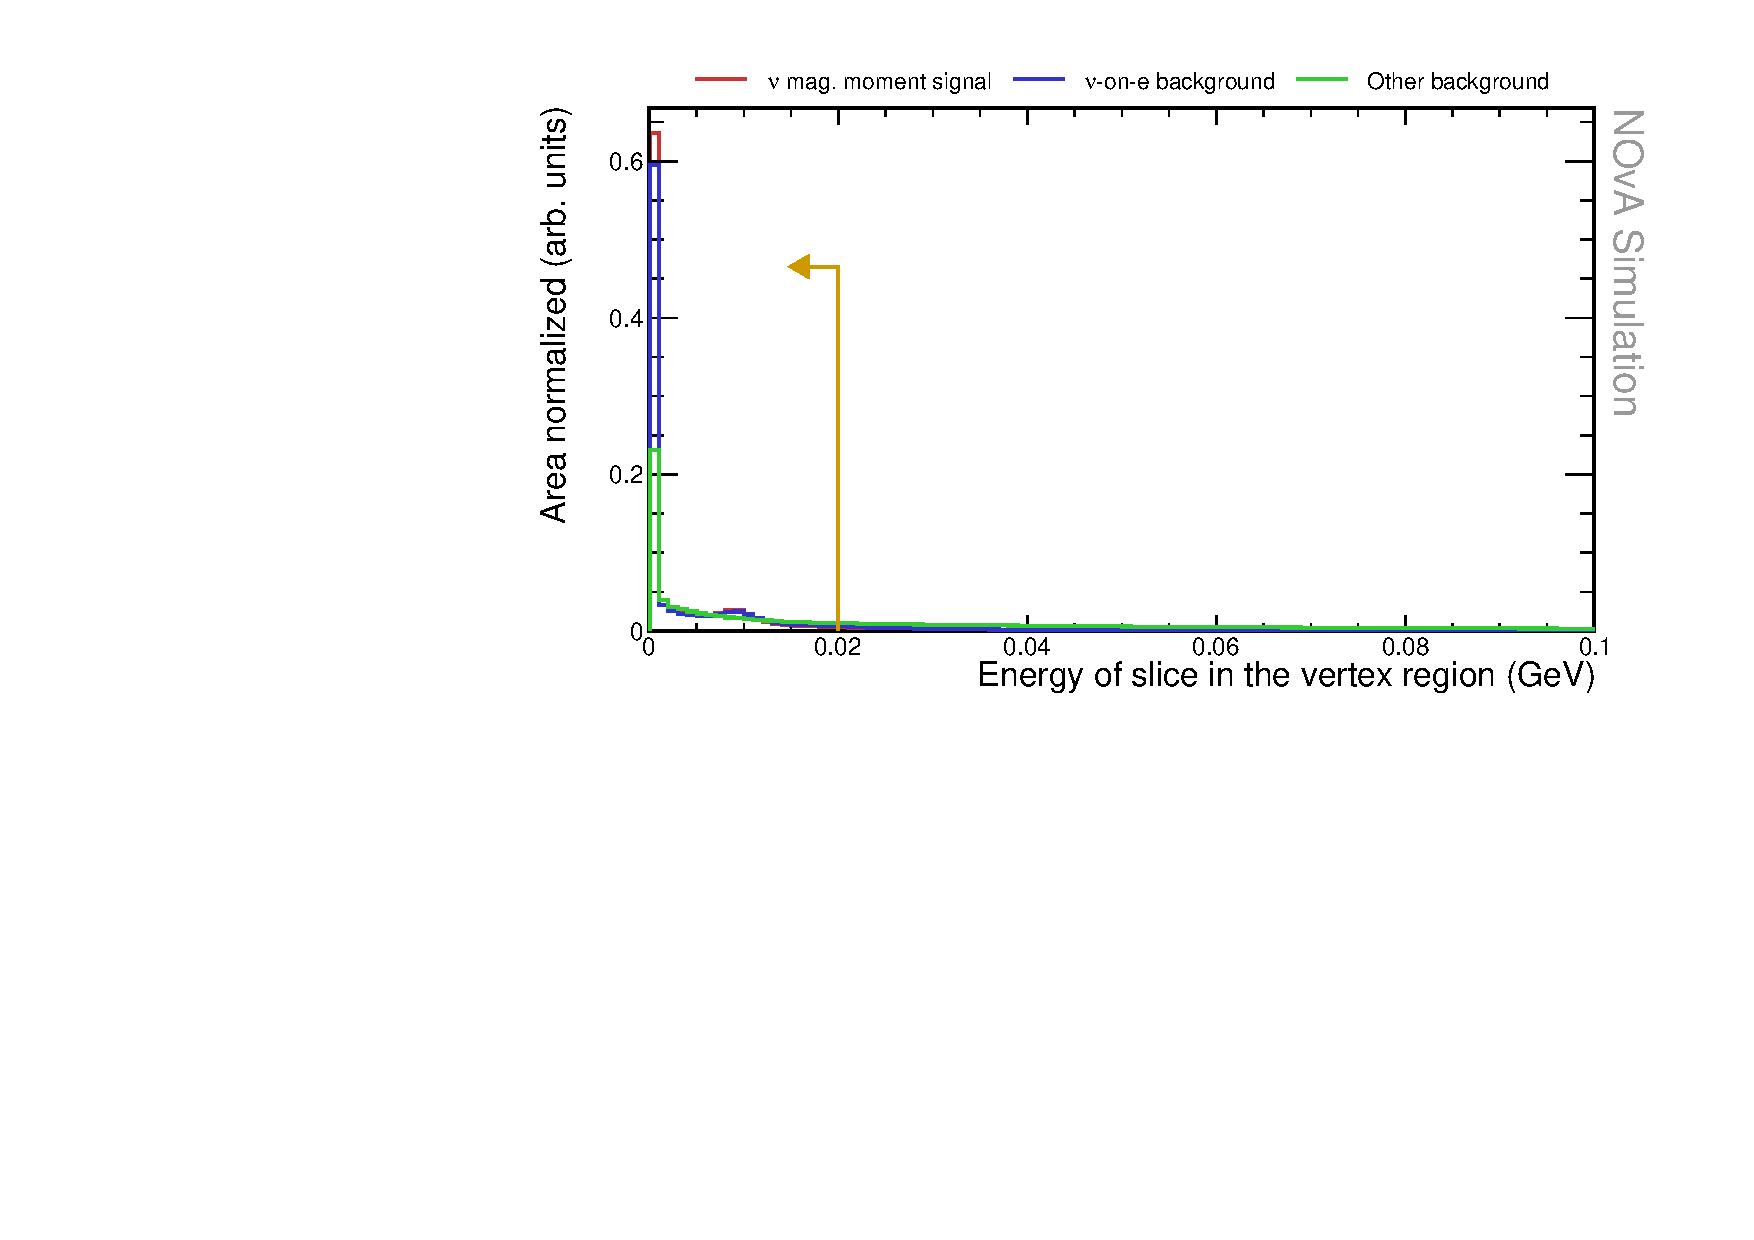
\includegraphics[width=.49\textwidth]{Plots/AnalysisOverview/N1Cut_vtxE.pdf}
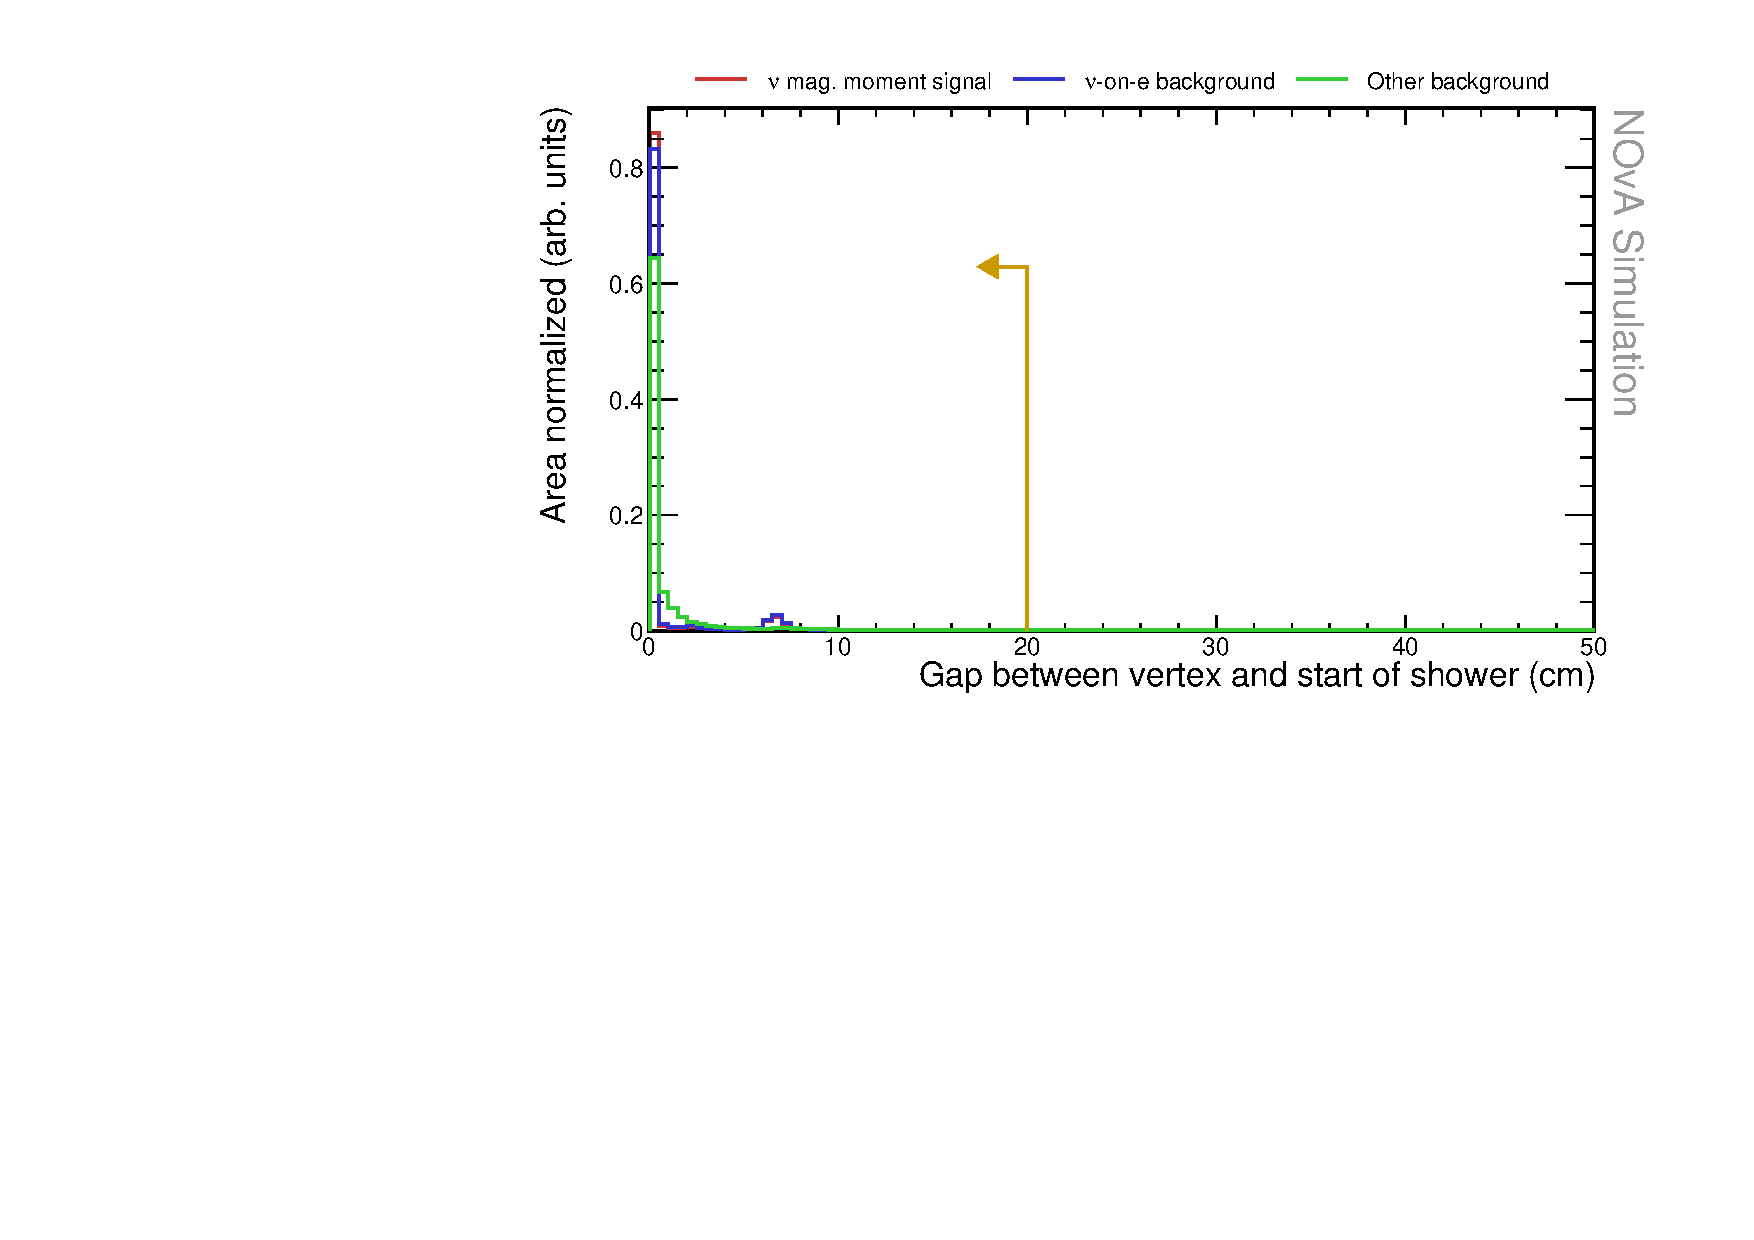
\includegraphics[width=.49\textwidth]{Plots/AnalysisOverview/N1Cut_gap.pdf}
\caption{Relative comparison of signal, $\nu$-on-e background, and other background events for the reconstructed vertex. No cuts were applied to make these plots. Gold lines show the cut values that create the fiducial volume.}
\label{fig:SingleShowerCuts}
\end{figure}

\subsubsection*{Shower energy cut}

\todo{discuss the energy cut, should this be removed? What is the effect on the event count? Why was this included in the first place (the identifiers are not as strong for lowere energies - is this true though? - also there are further unexplored backgrounds that would need to be further studied and explore. Maybe depends on where would we move the cut...)}
The calorimetric energy of the primary shower is required to be within $0.5<E_{cal}<5\ \unit{GeV}$.

\begin{figure}[hbtp]
\centering
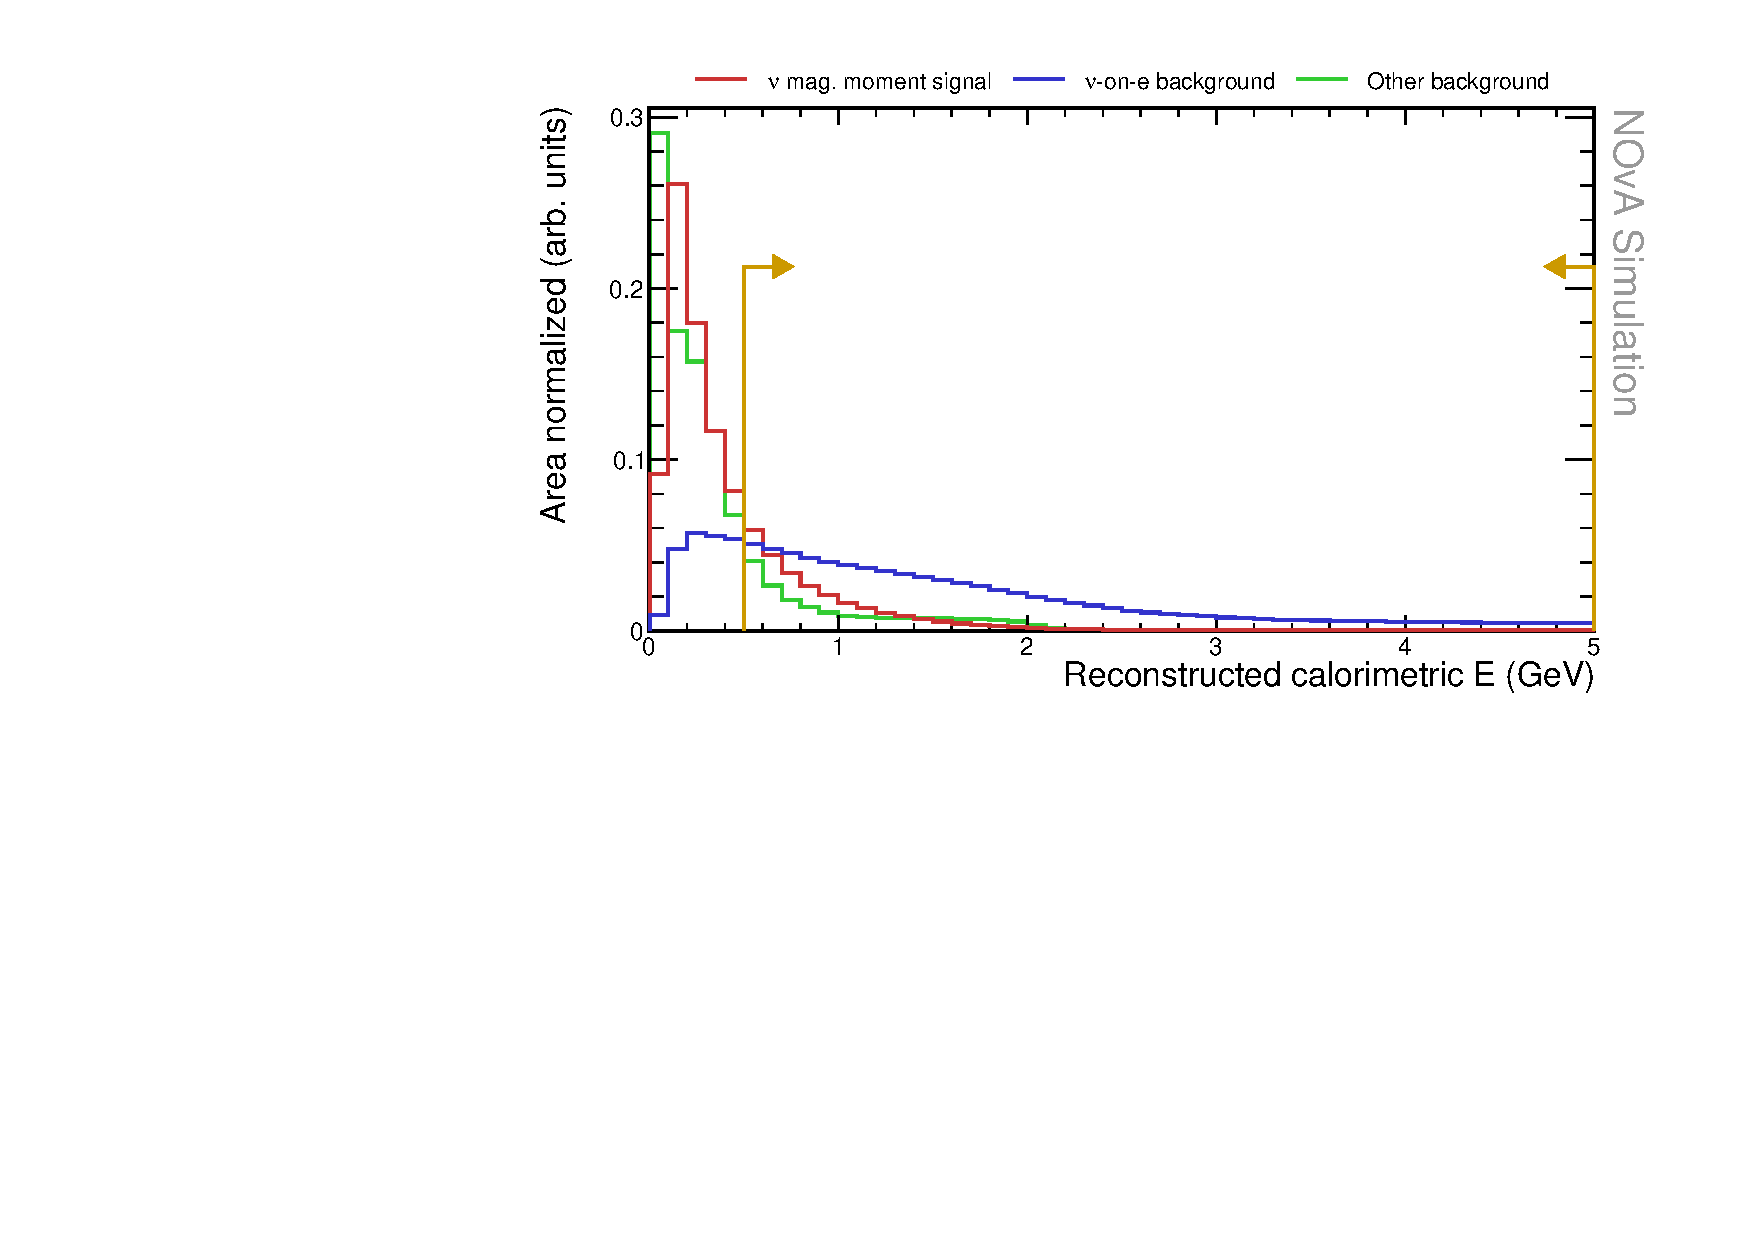
\includegraphics[width=.49\textwidth]{Plots/AnalysisOverview/N1Cut_calE.pdf}
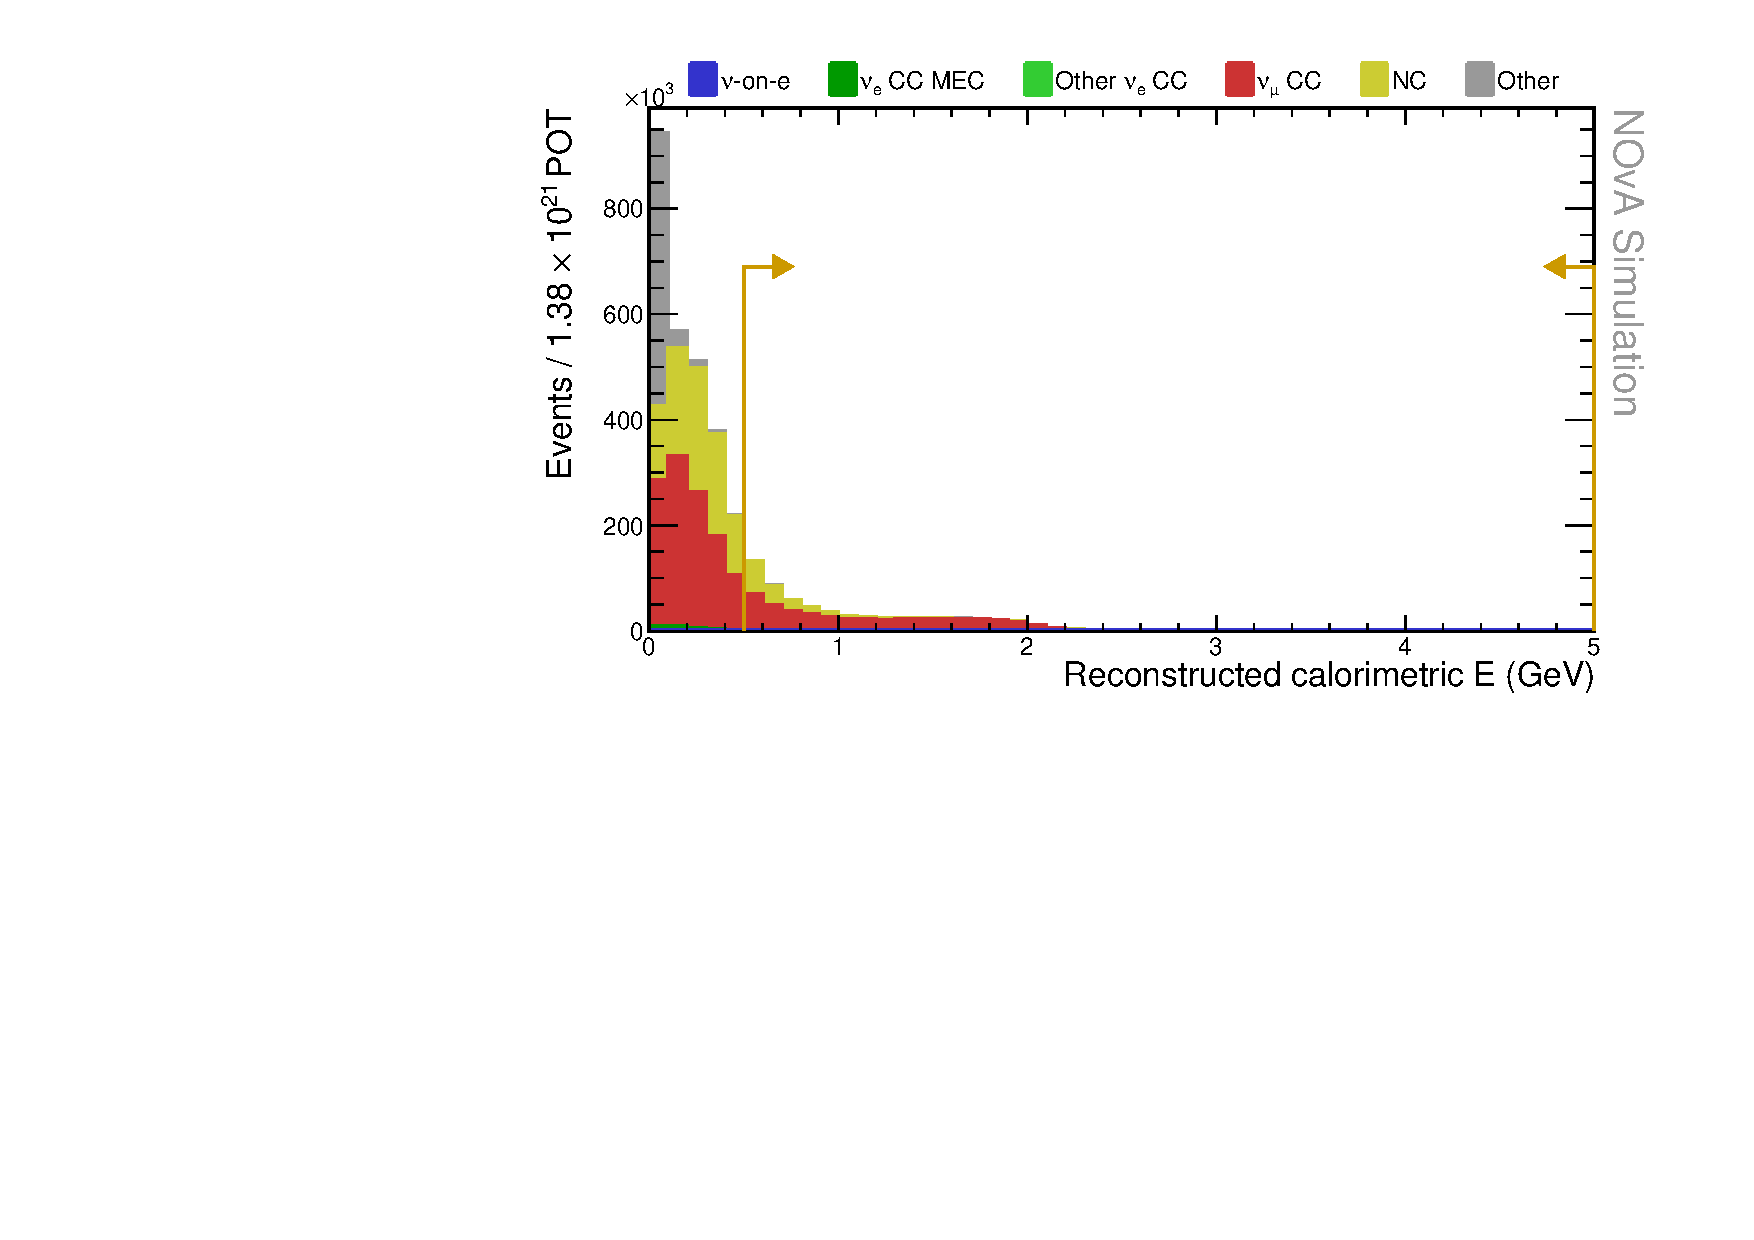
\includegraphics[width=.49\textwidth]{Plots/AnalysisOverview/N1Cut_calE_BkgDecomp.pdf}
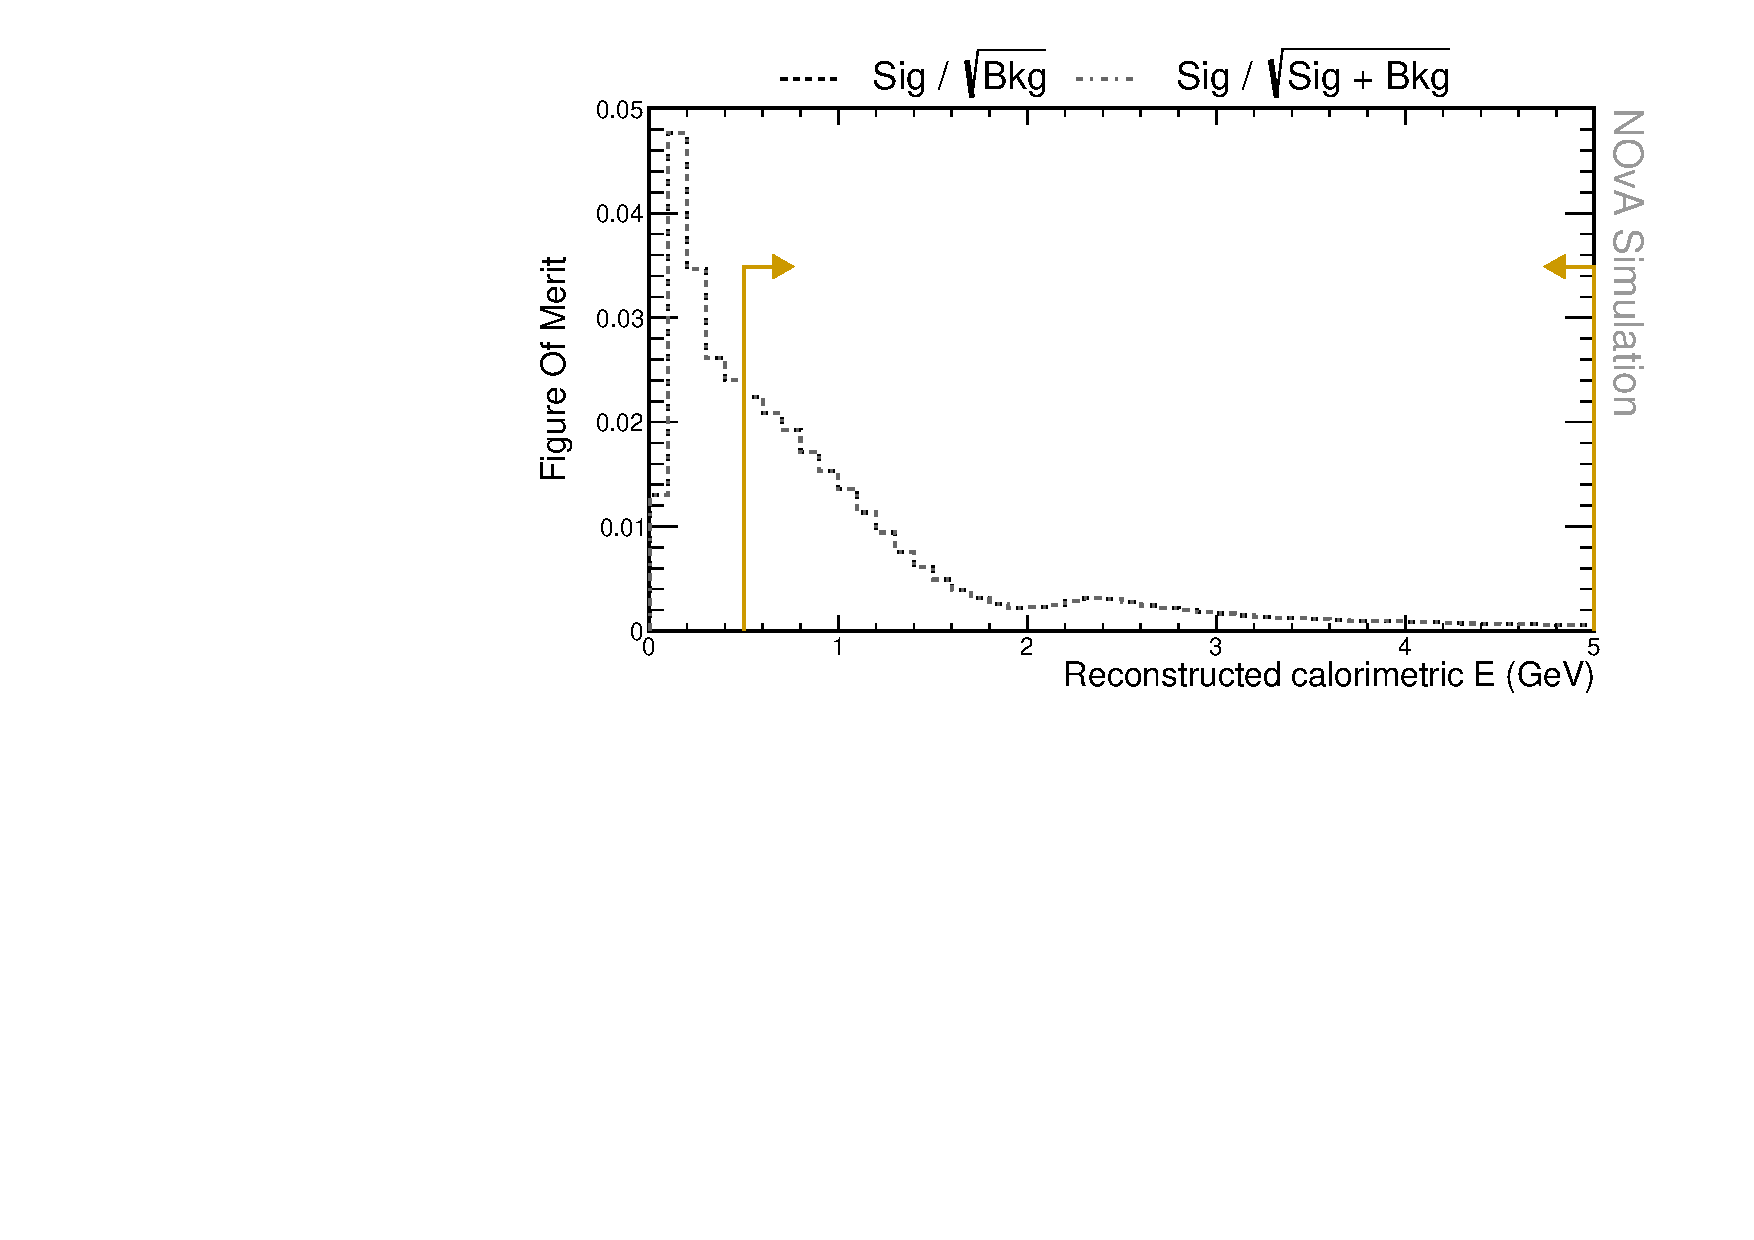
\includegraphics[width=.49\textwidth]{Plots/AnalysisOverview/NuMM_N1Cut_calE_Stat.pdf}
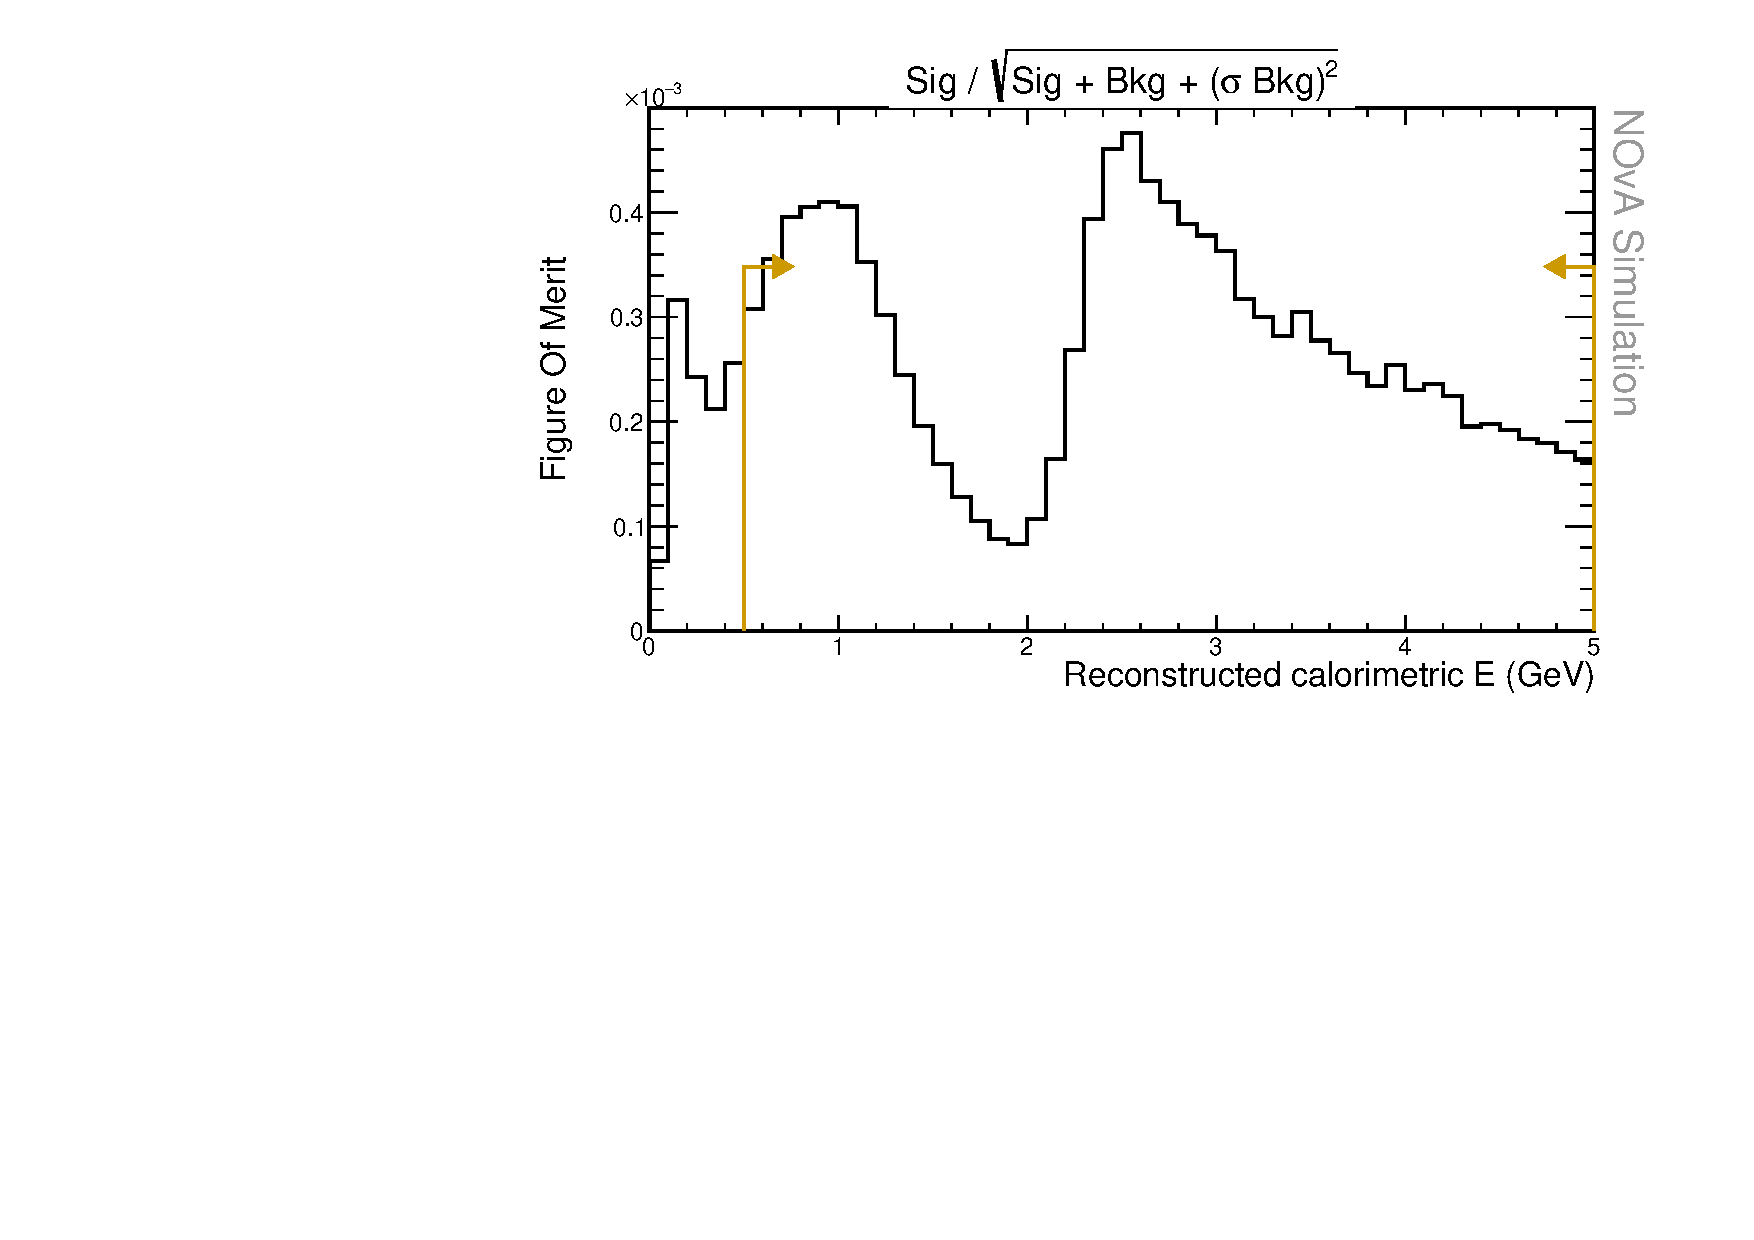
\includegraphics[width=.49\textwidth]{Plots/AnalysisOverview/NuMM_N1Cut_calE_Syst.pdf}
\caption{Relative comparison of signal, $\nu$-on-e background, and other background events for the reconstructed vertex. No cuts were applied to make these plots. Gold lines show the cut values that create the fiducial volume.}
\label{fig:SingleShowerCuts}
\end{figure}

\subsubsection*{Event classifiers}

We are using two event classifiers based on convolution neural network that were developed specifically to identify $\nu$-on-e interactions. The first one (\texttt{NuoneID}) is trained to select $\nu$-on-e events and the second one (\texttt{Epi0ID}) is trained on the events passing the \texttt{NuoneID} to reject the $\pi^0$ background. Our selection requires that \texttt{NuoneID}$>0.73$ and that \texttt{Epi0ID}$>0.92$.

\todo{reference theory for the kinematics of nuone scattering}
We require that the product of reconstructed energy of the primary shower and the square of its angle from the Z axis is $E_{cal}\theta^2<0.005\ \unit{GeV\times rad^2}$.

\todo{Add plots of distributions of the event selection variables with two columns. LHS shows no cuts applied and RHS shows all previous cuts applied}

Using the many plots below that show the effect of each of the cuts on the signal and all background events. (For signal we are showing NuMM=...)

\todo{Describe the cutflow tables below}
The final event count and efficiency of each of the cuts is shown on the table \ref{tab:CutflowTableSignal}. Table \ref{tab:CutflowTableBackground} shows the dissemination of background into the individual components.

\begin{table}[!hb]
\caption{Event selection cutflow table}
\begin{tabular}{|l|ccc|ccc|ccc|}\hline
\multicolumn{1}{|c|}{}                                     & \multicolumn{3}{c|}{\textbf{$\nu$ Mag. Moment signal}}          & \multicolumn{3}{c|}{\textbf{$\nu$-on-e background}}                      & \multicolumn{3}{c|}{\textbf{Other background}}                           \\
\multicolumn{1}{|c|}{\multirow{-2}{*}{\textbf{Selection}}} & \multicolumn{1}{c}{\textbf{$N_{sig}$}} & \textbf{$\epsilon^{N-1}$} & \textbf{$\epsilon \left(\%\right)$} & \multicolumn{1}{c}{\textbf{$N_{IBkg}$}} & \textbf{$\epsilon^{N-1}$} & \textbf{$\epsilon \left(\%\right)$} & \multicolumn{1}{c}{\textbf{$N_{Bkg}$}} & \textbf{$\epsilon^{N-1}$} & \textbf{$\epsilon \left(\%\right)$} \\\hline
\textbf{No Cut}      & 269.77            & 100 & 100 & 3.43$\times 10^3$           & 100 & 100                                     & 2.96$\times 10^8$          & 100                                                             & 100                                    \\
\textbf{Vtx Is Valid}  & 180.58            & 66.94                                                              & 66.94                                     & 3.33$\times 10^3$               & 96.94                                                               & 96.94                                      & 2.34$\times 10^8$          & 79.09                                                              & 79.09                                     \\
\textbf{N Prongs}        & 174.69            & 96.74                                                              & 64.76                                     & 3.23$\times 10^3$                             & 96.99                                                               & 94.02                                      & 8.66$\times 10^7$                     & 37.00                                                                 & 29.27                                     \\
\textbf{Png Length}  & 174.67            & 99.99                                                              & 64.75                                     & 3.22$\times 10^3$                                          & 99.64                                                               & 93.68                                      & 7.67$\times 10^7$                              & 88.56                                                              & 25.92                                     \\
\textbf{N Planes}      & 174.67            & 100                                                                & 64.75                                     & 3.22$\times 10^3$                                          & 99.98                                                               & 93.67                                      & 7.67$\times 10^7$          & 99.98                                                              & 25.92                                     \\
\textbf{N Cells}       & 174.67            & 100                                                                & 64.75                                     & 3.22$\times 10^3$                                           & 99.98                                                               & 93.65                                      & 7.42$\times 10^7$          & 96.78                                                              & 25.08                                     \\
\textbf{Closest Slc}  & 169.82            & 97.22                                                              & 62.95                                     & 3.14$\times 10^3$                                           & 97.54                                                               & 91.35                                      & 6.95$\times 10^7$          & 93.68                                                              & 23.49 \\
\textbf{Fiducial}     & 167.72            & 98.76                                                              & 62.17                                     & 3.09$\times 10^3$           & 98.41                                                               & 89.89                                      & 3.59$\times 10^7$          & 51.71                                                              & 12.15                                     \\
\textbf{Cont.}  & 159.37            & 95.02                                                              & 59.08                                     & 2.48$\times 10^3$           & 80.43                                                               & 72.30                                      & 1.38$\times 10^7$          & 38.35                                                              & 4.66                                      \\
\textbf{ShwE Frac.}  & 150.37            & 94.35                                                              & 55.74                                     & 2.42$\times 10^3$           & 97.59                                                               & 70.56                                      & 8.82$\times 10^6$          & 63.97                                                              & 2.98                                      \\
\textbf{Vtx E}         & 142.29            & 94.63                                                              & 52.74                                     & 2.18$\times 10^3$           & 90.16                                                               & 63.62                                      & 4.15$\times 10^6$          & 47.07                                                              & 1.40                                      \\
\textbf{Shw Gap}          & 137.96            & 96.96                                                              & 51.14                                     & 2.09$\times 10^3$           & 95.58                                                               & 60.80                                      & 3.25$\times 10^6$          & 78.34                                                              & 1.10                                      \\
\textbf{Shw E}      & 37.13             & 26.92                                                              & 13.76                                     & 1.36$\times 10^3$           & 65.10                                                               & 39.58                                      & 6.25$\times 10^5$          & 19.21                                                              & 0.21                                      \\
\textbf{Nuoneid}      & 29.48             & 79.39                                                              & 10.93                                     & 940.21             & 69.18                                                               & 27.38                                      & 2.42$\times 10^4$ & 3.88                                                               & 8.19$\times 10^{-3}$                                  \\
\textbf{Epi0id}       & 22.51             & 76.35                                                              & 8.34                                      & 749.93             & 79.76                                                               & 21.84                                      & 1.47$\times 10^4$ & 60.75                                                              & 4.97$\times 10^{-3}$                                  \\
\rowcolor[HTML]{67FD9A}
\textbf{$E\theta^2$}      & 19.74             & 87.73                                                              & 7.32                                      & 675.02             & 90.01                                                               & 19.66                                      & 84.15             & 0.57                                                               & 2.84$\times 10^{-5}$                                 \\\hline\hline
\textbf{$E\theta^2$ (sb)}  & 2.74              & -                                                              & 1.01                                      & 74.30              & -                                                               & 2.16                                       & 1.01$\times 10^3$          & - & 3.43$\times 10^{-4}$                                  \\\hline\hline
\textbf{No ShwE}  & 37.62             & -                                                           & 13.94                                     & 782.67             & -                                                            & 22.79                                      & 238.79            & -                                                              & 8.07E-05   \\\hline
\end{tabular}
\label{tab:CutflowTableSignal}
\end{table}

%\begin{landscape}
\begin{sidewaysfigure}[!hb]
\caption{Event selection cutflow table for background components}
\begin{scriptsize}
%\begin{table}[!hb]
\begin{tabular}{|l|ccc|ccc|ccc|ccc|ccc|}\hline
\multicolumn{1}{|c|}{\multirow{2}{*}{\textbf{Selection}}} & \multicolumn{3}{c|}{\textbf{$\nu_e$CC MEC}} &
\multicolumn{3}{c|}{\textbf{$\nu_e$CC Other}} &
\multicolumn{3}{c|}{\textbf{$\nu_\mu$CC}} &
\multicolumn{3}{c|}{\textbf{NC}} &
\multicolumn{3}{c|}{\textbf{Other}} \\
\multicolumn{1}{|c|}{}                                    & \multicolumn{1}{c}{\textbf{$N$}} & \textbf{$\epsilon^{N-1}$} & \textbf{$\epsilon \left(\%\right)$} & \multicolumn{1}{c}{\textbf{$N$}} & \textbf{$\epsilon^{N-1}$} & \textbf{$\epsilon \left(\%\right)$} & \multicolumn{1}{c}{\textbf{$N$}} & \textbf{$\epsilon^{N-1}$} & \textbf{$\epsilon \left(\%\right)$} & \multicolumn{1}{c}{\textbf{$N$}} & \textbf{$\epsilon^{N-1}$} & \textbf{$\epsilon \left(\%\right)$} & \multicolumn{1}{c}{\textbf{$N$}} & \textbf{$\epsilon^{N-1}$} & \textbf{$\epsilon \left(\%\right)$} \\\hline
\textbf{No Cut}      & 3.50$\times 10^4$           & 100 & 100                                     & 3.23$\times 10^6$             & 100 & 100 & 2.24$\times 10^8$              & 100                                                                 & 100                                        & 3.40$\times 10^7$          & 100.                                                             & 100                                    & 3.49$\times 10^7$                      & 100 & 100                                       \\
\textbf{Vtx Is Valid}  & 3.27$\times 10^4$           & 93.58                                                               & 93.58                                      & 2.62$\times 10^6$             & 81.14                                                                 & 81.14                                        & 1.99$\times 10^8$              & 89.02                                                                  & 89.02                                         & 2.57$\times 10^7$ & 75.55                                                              & 75.55                                     & 6.53$\times 10^6$             & 18.70                                                                 & 18.70                                        \\
\textbf{N Prongs}        & 2.74$\times 10^4$           & 83.76                                                               & 78.39                                      & 1.39$\times 10^6$             & 53.05                                                                 & 43.05                                        & 6.75$\times 10^7$              & 33.89                                                                  & 30.17                                         & 1.51$\times 10^7$          & 58.57                                                              & 44.25                                     & 2.65$\times 10^6$ & 40.51                                                                 & 7.58                                         \\
\textbf{Png Length}  & 2.73$\times 10^4$           & 99.79                                                               & 78.22                                      & 1.37$\times 10^6$             & 98.53                                                                 & 42.42                                        & 5.77$\times 10^7$ & 85.56                                                                  & 25.81                                         & 1.49$\times 10^7$          & 99.07                                                              & 43.84                                     & 2.64$\times 10^6$             & 99.87                                                                 & 7.57                                         \\
\textbf{N Planes}      & 2.73$\times 10^4$           & 99.99                                                               & 78.22                                      & 1.37$\times 10^6$             & 99.99                                                                 & 42.41                                        & 5.77$\times 10^7$              & 99.98                                                                  & 25.81                                         & 1.49$\times 10^7$          & 100                                                             & 43.84                                     & 2.64$\times 10^6$ & 100                                                                & 7.57                                         \\
\textbf{N Cells}       & 2.73$\times 10^4$           & 99.99                                                               & 78.21                                      & 1.28$\times 10^6$             & 93.49                                                                 & 39.65                                        & 5.59$\times 10^7$ & 96.82                                                                  & 24.98                                         & 1.44$\times 10^7$          & 96.34                                                              & 42.24                                     & 2.64$\times 10^6$             & 100                                                                & 7.57                                         \\
\textbf{Closest Slc}  & 2.73$\times 10^4$           & 99.79                                                               & 78.05                                      & 1.21$\times 10^6$ & 94.25                                                                 & 37.37                                        & 5.33$\times 10^7$ & 95.40                                                                  & 23.84                                         & 1.35$\times 10^7$          & 94.17                                                              & 39.77                                     & 1.43$\times 10^6$ & 54.22                                                                 & 4.10 \\
\textbf{Fiducial}     & 1.39$\times 10^4$           & 51.12                                                               & 39.90                                      & 6.30$\times 10^5$ & 52.10                                                                 & 19.47                                        & 2.60$\times 10^7$          & 48.77                                                                  & 11.62                                         & 8.25$\times 10^6$          & 60.99                                                              & 24.26                                     & 1.05$\times 10^6$             & 73.53                                                                 & 3.02                                         \\
\textbf{Cont.}  & 9.32$\times 10^3$           & 66.82                                                               & 26.66                                      & 2.63$\times 10^5$             & 41.72                                                                 & 8.12                                         & 7.64$\times 10^6$              & 29.38                                                                  & 3.42                                          & 4.96$\times 10^6$          & 60.15                                                              & 14.59                                     & 9.12$\times 10^5$             & 86.62                                                                 & 2.61                                         \\
\textbf{ShwE Frac.}  & 9.20$\times 10^3$           & 98.70                                                               & 26.32                                      & 1.95$\times 10^5$             & 74.39                                                                 & 6.04                                         & 4.82$\times 10^6$              & 63.10                                                                  & 2.15                                          & 2.97$\times 10^6$          & 59.78                                                              & 8.72                                      & 8.28$\times 10^5$             & 90.81                                                                 & 2.37                                         \\
\textbf{Vtx E}         & 5.92$\times 10^3$           & 64.33                                                               & 16.93                                      & 6.05$\times 10^4$             & 30.96                                                                 & 1.87                                         & 1.97$\times 10^6$ & 40.79                                                                  & 0.88                                          & 1.36$\times 10^6$          & 45.75                                                              & 3.99                                      & 7.62$\times 10^5$             & 92.03                                                                 & 2.18                                         \\
\textbf{Shw Gap}          & 5.50$\times 10^3$           & 92.91                                                               & 15.73                                      & 4.62$\times 10^4$             & 76.40                                                                 & 1.43                                         & 1.58$\times 10^6$ & 80.18                                                                  & 0.70                                          & 1.06$\times 10^6$          & 77.78                                                              & 3.10                                      & 5.69$\times 10^5$             & 74.61                                                                 & 1.63                                         \\
\textbf{Shw E}      & 3.62$\times 10^3$           & 65.81                                                               & 10.35                                      & 1.12$\times 10^4$             & 24.15                                                                 & 0.35                                         & 4.38$\times 10^5$              & 27.80                                                                  & 0.20                                          & 1.71$\times 10^5$          & 16.15                                                              & 0.50                                      & 1.28$\times 10^3$             & 0.23                                                                  & 3.68$\times 10^{-3}$                                     \\
\textbf{Nuoneid}      & 1.40$\times 10^3$           & 38.63                                                               & 4.00                                       & 2.11$\times 10^3$             & 18.89                                                                 & 0.065                                        & 1.17$\times 10^4$              & 2.66                                                                   & 5.21$\times 10^{-3}$                                      & 8.99$\times 10^3$          & 5.27                                                               & 0.026                                     & 66.43                & 5.17                                                                  & 1.90$\times 10^{-4}$                                     \\
\textbf{Epi0id}       & 1.14$\times 10^3$           & 81.78                                                               & 3.27                                       & 1.61$\times 10^3$             & 76.40                                                                 & 0.050                                        & 7.17$\times 10^3$              & 61.52                                                                  & 3.20$\times 10^{-3}$                                      & 4.76$\times 10^3$          & 52.94                                                              & 0.014                                     & 29.47                & 44.36                                                                 & 8.44$\times 10^{-5}$                                     \\
\rowcolor[HTML]{67FD9A}
\textbf{$E\theta^2$}      & 15.13              & 1.32                                                                & 0.043                                      & 39.00                & 2.42                                                                  & 1.21$\times 10^{-3}$                                     & 8.62                  & 0.12                                                                   & 3.85$\times 10^{-6}$                                      & 20.91             & 0.44                                                               & 6.15$\times 10^{-5}$                                  & 0.50                 & 1.69                                                                  & 1.43$\times 10^{-6}$                                  \\\hline\hline
\textbf{$E\theta^2$ (sb)}  & 386.16             & -                                                            & 1.10                                       & 306.55               & -                                                                & 9.48$\times 10^{-3}$                                     & 165.59                & -                                                               & 7.40$\times 10^{-5}$                                      & 149.93            & -                                                             & 4.41$\times 10^{-4}$                                  & 6.24                 & -                                                              & 1.79$\times 10^{-5}$                                     \\\hline\hline
\textbf{No ShwE}  & 15.54              & -                                                                & 0.044                                      & 69.61                & -                                                                 & 2.15$\times 10^{-3}$                                     & 68.48                 & - & 3.06$\times 10^{-5}$                                      & 75.67             & - & 2.22$\times 10^{-4}$                                  & 9.49                 & -                                                                & 2.72E-05   \\\hline
\end{tabular}

\label{tab:CutflowTableBackground}
%\end{table}
\end{scriptsize}
\end{sidewaysfigure}
%\end{landscape}

\todo{Add a discussion of possible improvements on the event selection on its limitations - mostly for the analysis review committee}
From here we can see that ... Maybe what can be improved is...
This can likely be improved upon by specifically selection low energy events and removing the cut on the reconstructed shower energy. 

\subsection{Resolution and binning}\label{sec:resolution}
\todo{Add the energy resolution and binning plots}
The electron energy and angle distributions and resolutions. Are we going to fit in E, Th, or ETh2? Is there something else?

Show plots of Reco V True for both energy and angle. (Should I show it with or without the energy cut?). Also show the resolution plots.

\subsection{Systematic uncertainties}
\todo{Describe the main systematic uncertainties. Add plots showing their effect on the NuMM events. Possibly with different event selection variables as X axes. Also show the final table with the percentages summed}
Plots showing combined uncertainties for signal and backgrounds. Maybe also some interpolations. Table of systematic uncertainties on the event count.

\subsubsection*{Normalization systematics}
\todo{Describe the normalization systematics (or just remove this if not using them in the end}
Should we include normalization systematics? Would that make any difference? There's a POT scaling uncertainty which is very small (find out exactly how small).

In the fitting experiment normalization uncertainties would probably not make any difference whatsoever, but in the counting experiment they might be important?

\subsubsection*{Neutrino flux systematics}
\todo{Describe the flux uncertainties. Describe the PCA. Describe the difference between what the ND group is doing and what we're doing}
Using the PCA vs using the PPFX universes+beam transport separately. Plots of energy showing shifts for signal and backgrounds separately

\todo{understand differences with ND and 3F methods}

This is mainly a normalization. Discuss how to use the fact that $\nu$-on-e events can be used (and are used) to constraint the beam uncertainty. Would the counting experiment still be valid then? Maybe if we made another sideband sample...

\subsubsection*{Detector systematics}
\todo{Make plots of energy showing shifts for signal and backgrounds separately}
Reference for the Prod5.1 detector systematics is docdb 53225

\subsubsection*{Cross section systematics}
\todo{Describe the XSec systs}
Only for the non nu-on-e background. Assuming the nu-on-e events (including the signal events) are precisely known.

Plots of energy showing shifts for signal and backgrounds separately

\subsection{Fitting framework}
\todo{Describe the fitting framework, ideally with an example plot, maybe with some arrows}
How does the fitting framework work? It's based on the framework developed by Mu Wei for the Light Dark Matter analysis (ref.) which was developed together (is this fair?). Basic description of the framework.

Also this framework is used for both LDM and NuMM together. It is trivial to simply switch between including the NuMM or LDM in it. This was done to save space in creating predictions since our backgrounds are exactly the same (or at least they should be...). Theoretically this could be separated into two difference frameworks.

\begin{itemize}
\item <NDPredictionSingleElectron> Prediction class which holds the LDM as a special 2-D spectrum (not used for NuMM), and NuMM, $\nu$-on-e background, $\nu_e$CC MEC background and other background as simple 1-D spectra. Also scaling each spectra by...
\item <NDPredictionSystSingleElectron> class derived from PredictionInterp that takes in the NDPredictionSingleElectron and applies systematic shifts to it. Includes the interpolation/extrapolation between the systematic shifts.
\item FitVariables and what do they do
\item Fitter which does exactly what... What are the parameters of the fit? What are the results/outputs?
\end{itemize}